\chapter{Dinamica del Punto Materiale}
La dinamica studia il movimento dei corpi in relazione alle cause che lo modificano, ovvero alle \textbf{FORZE}.
Nella dinamica le grandezze fisiche fondamentali che entrano in gioco sono:
\begin{enumerate}
    \item Lunghezza $[L]$
    \item Tempo $[T]$
    \item Massa $[M]$
\end{enumerate}

\section{La Forza (Definizione Generale)}
In generale, la \textbf{Forza} è definita come un'\textbf{INTERAZIONE} fra corpi.
Tutti i tipi di forze condividono alcune proprietà fondamentali:
\begin{enumerate}
    \item \textbf{Grandezze Vettoriali}: sono descritte da un modulo, una direzione e un verso.
    \item \textbf{Principio di Sovrapposizione}: vige l'indipendenza delle azioni simultanee. Se più forze agiscono su un corpo, la forza totale è la somma vettoriale delle singole forze: $\vec{F}_{tot} = \sum \vec{F}_i$.
    \item \textbf{Dipendenza dalla Distanza}: tendenzialmente il modulo della forza $|\vec{F}|$ diminuisce all'aumentare della distanza $d$ tra i corpi (spesso $|\vec{F}| \propto d^{-2}$).
    \item \textbf{Indipendenza dal Sistema di Riferimento}: la forza $\vec{F}$ è invariante per trasformazioni di Galileo (non cambia al variare del riferimento inerziale), così come non cambiano la distanza, il modulo della velocità relativa $|\vec{v}_{rel}|$, la massa e la carica.
\end{enumerate}

\section{Tipologie di Forze}
Esistono diversi tipi di forze, classificabili in due grandi categorie:

\subsection{Forze A Distanza (Fondamentali)}
Agiscono senza contatto diretto tra i corpi:
\begin{itemize}
    \item Forza Gravitazionale.
    \item Forza Elettromagnetica.
    \item Forze Nucleari (Forte e Debole) e Atomiche.
\end{itemize}

\subsection{Forze Di Contatto}
Sono manifestazioni macroscopiche delle forze fondamentali (principalmente elettromagnetiche) che si generano dal contatto tra superfici.

\begin{figure}[ht]
    \centering
    \begin{tikzpicture}[
        grow=right,
        level 1/.style={sibling distance=3.2cm, level distance=4.5cm},
        level 2/.style={sibling distance=1.8cm, level distance=5.5cm},
        edge from parent/.style={draw, thick, -stealth},
        every node/.style={font=\small},
        box/.style={draw, rounded corners, minimum height=0.9cm, minimum width=2.2cm, align=center, font=\small},
        leaf/.style={draw, rounded corners=3pt, fill=gray!8, minimum height=0.8cm, align=center, font=\small}
    ]
    \node[box, fill=mypen!15, font=\bfseries] {Forze di Contatto}
        child { 
            node[box, fill=green!15] {Rigido--Fluido}
            child { node[leaf] {\textbf{Attrito Viscoso}} }
            child { node[leaf] {\textbf{Pressione}} }
        }
        child { 
            node[box, fill=orange!15] {Deformabile--Def.}
            child { node[leaf] {\textbf{Anelastiche}} }
            child { node[leaf] {\textbf{Elastiche}} }
        }
        child { 
            node[box, fill=red!15] {Rigido--Rigido}
            child { node[leaf] {\textbf{Attrito} \\ \scriptsize{Statico, Dinamico}} }
            child { node[leaf] {\textbf{Vincolari} \\ \scriptsize{Tensioni, Reazioni}} }
        };
    \end{tikzpicture}
    \caption{Classificazione delle Forze di Contatto.}
\end{figure}

\section{Misurazione delle Forze}
La misurazione delle forze può avvenire in due modi principali:

\begin{enumerate}[label=\alph*)]
    \item \textbf{Misura Dinamica}:
    È una misura indiretta. Conoscendo la massa $m$ del corpo e potendo misurare la sua accelerazione $\vec{a}$, si sfrutta la seconda legge della dinamica:
    \[ \vec{F} = m \cdot \vec{a} \]
    
    \item \textbf{Misura Statica}:
    È una misura diretta basata sull'equilibrio. Si bilancia una forza nota $F_n$ con la forza incognita $F_i$, oppure si rapportano le deformazioni (lunghezze) causate dalle forze.
    
    Strumenti tipici:
    \begin{itemize}
        \item \textbf{Dinamometro}: Sfrutta la deformazione elastica di una molla ($F = k \Delta x$).
        \item \textbf{Bilancia}: Sfrutta l'equilibrio dei momenti o delle forze peso.
    \end{itemize}
    
    \begin{center}
    \begin{tikzpicture}[scale=0.8]
        % Dinamometro
        \begin{scope}[yshift=0cm]
             \draw[thick] (-0.5, 3) -- (0.5, 3);
             \draw[decoration={aspect=0.3, segment length=2mm, amplitude=2mm, coil}, decorate] (0, 3) -- (0, 1);
             \draw[->, thick] (0, 1) -- (0, 0) node[right] {$\vec{F}$};
             \draw (-0.2, 1) -- (0.2, 1); 
             \node[left] at (-0.5, 2) {\small Dinamometro};
        \end{scope}

        % Bilancia
        \begin{scope}[xshift=6cm]
            \draw[thick] (0, 0) -- (0, 2.5); % Piatto centrale
            \draw[thick] (-2, 2.5) -- (2, 2.5); % Braccio
            \draw (-2, 2.5) -- (-2, 1.5); % Filo sx
            \draw (-2.4, 1.5) -- (-1.6, 1.5); % Piatto sx
            
            \draw (2, 2.5) -- (2, 1.5); % Filo dx
            \draw (1.6, 1.5) -- (2.4, 1.5); % Piatto dx
            
            \filldraw (0, 2.5) circle (2pt); % Fulcro
            \node at (0, -0.5) {\small Bilancia};
        \end{scope}
    \end{tikzpicture}
    \end{center}
\end{enumerate}

\section{Principi della Dinamica}
I principi della dinamica furono enunciati formalmente da \textbf{Isaac Newton} nella sua opera monumentale \textit{"Philosophiae Naturalis Principia Mathematica"} (1687), riprendendo e sistematizzando gli studi precedenti di \textbf{Galileo Galilei}.

\subsection{Primo Principio: Principio di Inerzia}
\begin{definizione}{Primo Principio: Principio di Inerzia}
Un corpo permane nel suo stato di quiete o di moto rettilineo uniforme finché non interviene una forza esterna a variarne lo stato.
\[ \sum \vec{F} = 0 \implies \vec{v} = \text{cost} \]
Questa proprietà intrinseca della materia è detta \textbf{Inerzia}.
\end{definizione}

Pertanto, se la risultante delle forze è nulla ($\vec{F}_{tot} = 0$), il corpo si trova in uno degli \textbf{Stati di Equilibrio}:
\begin{itemize}
    \item \textbf{Quiete} ($v=0$).
    \item \textbf{Moto Rettilineo Uniforme} ($v = \text{cost} \neq 0$).
\end{itemize}

La condizione $\vec{F}_{tot} = 0$ si verifica in due casi esclusivi:
\begin{enumerate}[label=\alph*)]
    \item Il corpo non è soggetto ad alcuna forza ($F=0$).
    \item Il corpo è soggetto a più forze la cui somma vettoriale è nulla ($\sum \vec{F} = 0$).
\end{enumerate}

\begin{esercizio}{Il Paradosso Sperimentale e l'Esperimento Ideale di Galileo}
A livello concreto, è impossibile osservare il principio di inerzia in forma pura sulla Terra, poiché non otteniamo mai una reale prova sperimentale dell'assenza completa di forze. Infatti, le forze dissipative (come l'attrito dell'aria o del piano) sono sempre presenti.

Per risolvere questo paradosso, Galileo ideò un celebre \textbf{Esperimento Intellettuale} (\textit{Gedankenexperiment}):

    \begin{center}
    \begin{tikzpicture}[scale=0.85, transform shape] 
        % --- Caso A: Simmetrico Ripido ---
        \begin{scope}[xshift=-4cm, yshift=2.5cm]
            \coordinate (TopLeft) at (-2, 2);
            \coordinate (Bottom) at (0, 0);
            \coordinate (TopRight) at (2, 2);
            \draw[thick, rounded corners=15pt] (TopLeft) -- (Bottom) -- (TopRight);
            \draw[dashed, gray] (TopLeft) -- (TopRight);
            \draw[thick] (-2,0) -- (2,0);
            \draw[thick] (-2,2) -- (-2,0);
            \draw[thick] (2,2) -- (2,0);
            \node[left] at (-2.2, 1) {\textbf{A}};
            \node[right, gray] at (TopRight) {$h$};
            \coordinate (BallDown) at (-1.2, 1.2);
            \filldraw[fill=gray!30, draw=black] (BallDown) circle (0.18);
            \draw[->, thick] (BallDown) -- ++(-45:0.8);
            \coordinate (BallUp) at (1.2, 1.2);
            \filldraw[fill=gray!30, draw=black] (BallUp) circle (0.18);
            \draw[->, thick] (BallUp) -- ++(45:0.8);
        \end{scope}
        
        % --- Caso B: Simmetrico Largo ---
        \begin{scope}[xshift=4cm, yshift=2.5cm]
            \coordinate (TopLeftB) at (-3.5, 2);
            \coordinate (BottomB) at (0, 0);
            \coordinate (TopRightB) at (3.5, 2);
            \draw[thick, rounded corners=20pt] (TopLeftB) -- (BottomB) -- (TopRightB);
            \draw[dashed, gray] (TopLeftB) -- (TopRightB);
            \draw[thick] (-3.5,0) -- (3.5,0);
            \draw[thick] (-3.5,2) -- (-3.5,0);
            \draw[thick] (3.5,2) -- (3.5,0);
            \node[left] at (-3.7, 1) {\textbf{B}};
            \node[right, gray] at (TopRightB) {$h$};
            \coordinate (BallDownB) at (-2, 1.14);
            \filldraw[fill=gray!30, draw=black] (BallDownB) circle (0.18);
            \draw[->, thick] (BallDownB) -- ++(-29.7:0.8);
            \coordinate (BallUpB) at (2, 1.14);
            \filldraw[fill=gray!30, draw=black] (BallUpB) circle (0.18);
            \draw[->, thick] (BallUpB) -- ++(29.7:0.8);
        \end{scope}
        
        % --- Caso C: Piano Orizzontale ---
        \begin{scope}[xshift=0cm, yshift=-1.5cm]
            \draw[thick] (-4, 0) -- (4, 0);
            \draw[->, thick, dashed] (4, 0) -- (5.5, 0); 
            \node[left] at (-4.2, 0.5) {\textbf{C}};
            \filldraw[fill=gray!30, draw=black] (0, 0.18) circle (0.18);
            \draw[->, thick, mygreen] (0.3, 0.18) -- (1.8, 0.18) node[above] {$\vec{v} = \text{cost}$};
            \node[below, mygreen] at (1.5, -0.2) {MRU};
        \end{scope}
    \end{tikzpicture}
    \captionof{figure}{Esperimento dei piani inclinati di Galileo.}
    \end{center}

Immaginando di avere due piani inclinati contrapposti:
\begin{enumerate}
    \item Il corpo scivola sul primo piano \textbf{accelerando} e risale sul secondo \textbf{decelerando} fino a tornare alla quota iniziale $h$.
    \item Riducendo l'inclinazione del secondo piano, il corpo percorre un tratto più lungo.
    \item Se l'inclinazione del secondo piano diventa \textbf{nulla} (piano orizzontale), il corpo continuerà a muoversi indefinitamente a velocità costante (\textbf{MRU}).
\end{enumerate}
\end{esercizio}

\subsection{Sistemi di Riferimento Inerziali}
Un altro fatto fondamentale è legato alla relatività del moto.
Infatti:
\begin{itemize}
    \item \textbf{Caso A (Sistemi Fermi/Inerziali)}: Se l'osservatore è fermo, vede i corpi liberi (su cui non agiscono forze) muoversi di MRU o stare fermi.
    \item \textbf{Caso B (Sistemi Accelerati)}: Se l'osservatore si trova in un sistema accelerato (es. su una giostra in rotazione, $\omega \neq 0$), vedrà i corpi muoversi di moto accelerato (forze apparenti) anche se su di essi non agisce alcuna forza reale. In questo caso il Primo Principio \textbf{NON} è valido.
\end{itemize}

\begin{definizione}{Sistemi di Riferimento Inerziali}
Si definisce \textbf{Inerziale} un sistema di riferimento in cui vale il Primo Principio della Dinamica. Tutti i sistemi in moto rettilineo uniforme rispetto a un sistema inerziale sono anch'essi inerziali (\textbf{Classe di Inerzialità}).
\end{definizione}

\subsubsection{Proprietà dei Sistemi Inerziali}
\begin{enumerate}
    \item \textbf{Classe di Equivalenza}: Sono inerziali tutti e soli i sistemi che si muovono di \textbf{MRU} rispetto ad un sistema inerziale $S$.
    \item \textbf{Transitivitá}: Se $S$ è inerziale e $S'$ è in MRU rispetto a $S \Rightarrow S'$ è inerziale.
    \item \textbf{Le Stelle Fisse}: Un sistema di riferimento solidale con le "stelle fisse" (stelle enormemente lontane, percepite come "ferme") è un'ottima approssimazione di sistema inerziale.
    \item \textbf{Relatività di Galileo}: Le leggi della meccanica sono le stesse in \textbf{tutti} i sistemi di riferimento inerziali. Non esiste un sistema inerziale privilegiato.
\end{enumerate}

\begin{osservazione}{La Terra è un sistema inerziale?}
Rigorosamente \textbf{NO}, a causa dei moti di rotazione e rivoluzione. Tuttavia, per la maggior parte delle applicazioni locali, può essere approssimata come tale poiché queste accelerazioni sono trascurabili rispetto a $g$.
\end{osservazione}
Tuttavia, può essere considerata \textbf{approssimativamente inerziale} per la maggior parte degli esperimenti di laboratorio, poiché tali accelerazioni sono molto piccole rispetto alla gravità:
\[ a_{rot} \approx 2.5 \cdot 10^{-3} g, \quad a_{riv} \approx 10^{-4} g \]
Questi effetti diventano rilevanti solo per moti su grande scala (es. correnti atmosferiche) o misure di altissima precisione.

\section{Secondo Principio: Legge Fondamentale (Legge di Newton)}

% ---------------------------------------------------------------
\subsection{Prima Formulazione (Massa Costante)}
% ---------------------------------------------------------------

\noindent
\begin{minipage}[t]{0.52\textwidth}
\vspace{0pt}
dove $\sum\vec{F}$ è la somma delle forze applicate
ad un corpo, avente la stessa direzione dell'accelerazione
$\vec{a}$; la costante di proporzionalità è la massa $m$:
\begin{equation}\label{eq:2nd_law}
    \boxed{\sum \vec{F} = m \cdot \vec{a}}
\end{equation}
\end{minipage}%
\hfill
\begin{minipage}[t]{0.44\textwidth}
\vspace{4pt}
\begin{osservazione}{Unità di misura della Forza}
Nel Sistema Internazionale, la forza si misura in \textbf{Newton} [N]:
\[ 1 \, N = 1 \, kg \cdot m/s^2 \]
\end{osservazione}
\end{minipage}

\medskip
\begin{osservazione}{Relazione tra i Principi}
Affinché valga il 2° principio è necessario definire un sistema di riferimento inerziale tramite il 1° principio. In sistemi non inerziali compaiono forze apparenti che invalidano la forma $\sum \vec{F} = m\vec{a}$ se non corrette.
\end{osservazione}

\begin{definizione}{Secondo Principio della Dinamica}
In un sistema di riferimento \textbf{inerziale}, l'accelerazione di
un punto materiale è \emph{direttamente proporzionale} alla forza
risultante e \emph{inversamente proporzionale} alla sua massa:
\[
    \vec{a} = \vec{R} \;\Longrightarrow\;
    \vec{a} = \frac{\sum\vec{F}}{m} \;\Longrightarrow\;
    \underbrace{\frac{\sum\vec{F}(\vec{r},\dot{\vec{r}})}{m}
               = \ddot{\vec{r}}}_{\text{equazione del moto}}
\]
\end{definizione}

\paragraph{Equazioni Scalari.}
Essendo un'equazione vettoriale, equivale a tre equazioni scalari:
\[
\begin{cases}
    \sum F_x = m\, a_x \\
    \sum F_y = m\, a_y \\
    \sum F_z = m\, a_z
\end{cases}
\qquad\text{con }\; a_i = \dfrac{d^2 x_i}{dt^2}
\]

\paragraph{Problemi della Dinamica.}
\begin{itemize}
    \item \textbf{Diretto}: note forze e c.i.\ ($\vec{r}_0,\vec{v}_0$)
          $\;\ \to\;$ trovare $\vec{r}(t)$.
    \item \textbf{Inverso}: noto $\vec{r}(t)$ (e quindi $\vec{a}$)
          $\;\ \to\;$ trovare le forze.
\end{itemize}

% ---------------------------------------------------------------
\subsection{Formulazione Generale di Newton (Quantità di Moto)}
% ---------------------------------------------------------------
Newton fornì una definizione più generale introducendo la
\textbf{quantità di moto} $\vec{p} = m\vec{v}$.
Per $m = \text{costante}$:
\[
    \sum \vec{F} = \frac{d\vec{p}}{dt}
    \qquad\text{poiché}\qquad
    \frac{d\vec{p}}{dt} = m\frac{d\vec{v}}{dt} = m\vec{a}
\]

\begin{teorema}{Secondo Principio — Forma Generale}
In un sistema inerziale, per un punto materiale con
$\vec{p} = m\vec{v}$:
\begin{equation}\label{eq:2nd_general}
    \sum \vec{F} = \frac{d\vec{p}}{dt}
\end{equation}
Questa forma è valida anche per sistemi a \textbf{massa variabile}
(es.\ un razzo che espelle carburante).
\end{teorema}

\smallskip
Sfruttare $\vec{p}$ risulta efficace in: studio di sistemi multi-corpo,
moto rapidi (urti fra particelle), sistemi a massa variabile.

% ---------------------------------------------------------------
\subsection{Teorema dell'Impulso}
% ---------------------------------------------------------------
\begin{teorema}{Teorema dell'Impulso}
L'impulso della forza/sistema di forze è uguale alla variazione della
quantità di moto del corpo su cui agisce.
Integrando $\sum\vec{F}$ tra $t_1$ e $t_2$:
\begin{align*}
    \vec{I}_{t_1 \to t_2}
        &= \int_{t_1}^{t_2}\sum\vec{F}\,dt
         = \int_{t_1}^{t_2}\frac{d\vec{p}}{dt}\,dt
         = \int_{t_1}^{t_2}d\vec{p} 
        = \bigl[\vec{p}\bigr]_{t_1}^{t_2}
         = \vec{p}(t_2)-\vec{p}(t_1)
         = \Delta\vec{p}
\end{align*}
\end{teorema}

% ---------------------------------------------------------------
\subsubsection{Forze Impulsive}
% ---------------------------------------------------------------
\noindent
Le forze ``impulsive'' (es.\ urto) sono \textbf{molto intense} e
agiscono per un \textbf{breve intervallo} $\Delta t\approx 1\,\mathrm{ms}$.\medskip

\noindent
Sfruttando il teorema dell'impulso, la \textbf{forza impulsiva media}
è definita come:
\begin{align*}
    \int_{0^-}^{0^+}\vec{F}\,dt
        &= \langle\vec{F}\rangle_{\Delta t}\cdot\Delta t
         = \vec{p}(0^+)-\vec{p}(0^-)
    \Longrightarrow\quad
    \boxed{\langle\vec{F}\rangle_{\Delta t} = \frac{\Delta\vec{p}}{\Delta t}}
    \qquad\text{(media integrale)}
\end{align*}

\noindent
Analizziamo gli stati immediatamente prima ($t=0^-$) e dopo ($t=0^+$) dell'urto:

\begin{figure}[ht]
    \centering
    \begin{tikzpicture}[scale=1.05, >=stealth]
        % Muro verticale con tratteggio
        \draw[line width=3pt, color=darkgray] (0,-1.8) -- (0,1.8);
        \fill[pattern=north east lines, pattern color=gray!70]
            (-0.35,-1.8) rectangle (0,1.8);
        \node[above, color=darkgray, font=\small\itshape] at (0,1.85)
            {Parete Rigida};

        % --- PRIMA DELL'URTO (t = 0-) ---
        \begin{scope}[yshift=0.9cm]
            \node[circle, draw=gray!70, dashed, minimum size=1.1cm,
                  thick, fill=gray!8] (ball_in) at (2.2, 0) {};
            \node[gray, font=\small] at (2.2, 0) {$m$};
            \draw[->, thick, gray] (ball_in.west) -- ++(-1.2,0)
                node[midway, above, font=\small] {$\vec{v}_{in}$};
            \node[right, gray!80, font=\footnotesize] at (2.9,0) {$t=0^-$};
        \end{scope}

        % --- DURANTE L'URTO (t = 0): forza impulsiva ---
        \fill[red!80] (0,0) circle (2.5pt);
        \draw[->, ultra thick, red!80] (0,0) -- (1.8,0)
            node[midway, below, font=\small] {$\vec{F}_{imp}$};
        \node[left, red!80, font=\footnotesize] at (-0.05,0) {$t=0$};

        % --- DOPO L'URTO (t = 0+) ---
        \begin{scope}[yshift=-0.9cm]
            \node[circle, draw=black, fill=white, minimum size=1.1cm,
                  thick] (ball_out) at (2.2, 0) {};
            \node[font=\small] at (2.2, 0) {$m$};
            \draw[->, thick, black] (ball_out.east) -- ++(1.2,0)
                node[midway, above, font=\small] {$\vec{v}_{out}$};
            \node[right, black, font=\footnotesize] at (2.9,-0.4) {$t=0^+$};
        \end{scope}
    \end{tikzpicture}
    \caption{Urto elastico contro una parete rigida. La forza impulsiva
        $\vec{F}_{imp}$ agisce per $\Delta t\to 0$, causando la variazione
        di quantità di moto $\Delta\vec{p} = \vec{p}(0^+)-\vec{p}(0^-)$.}
    \label{fig:impulso}
\end{figure}

\section{Terzo Principio: Azione e Reazione}
\begin{definizione}{Terzo Principio: Azione e Reazione}
Se un corpo $A$ esercita una forza $\vec{F}_{AB}$ su un corpo $B$, il corpo $B$ esercita contemporaneamente una forza $\vec{F}_{BA}$ su $A$, tale che:
\begin{equation}
    \vec{F}_{AB} = -\vec{F}_{BA}
\end{equation}
Le due forze hanno stessa retta d'azione, stesso modulo, ma versi opposti. Si applicano a \textbf{punti materiali diversi}.
\end{definizione}
Questo significa che le forze di interazione ("Azione" e "Reazione") compaiono sempre in \textbf{coppia} e condividono le seguenti caratteristiche:
\begin{itemize}
    \item Hanno lo stesso \textbf{modulo}: $|\vec{F}_{AB}| = |\vec{F}_{BA}|$.
    \item Hanno la stessa \textbf{direzione} (la retta congiungente i due corpi).
    \item Hanno \textbf{verso opposto}.
    \item \textbf{Agiscono su corpi DIVERSI}:
    \begin{itemize}
        \item $\vec{F}_{AB}$ agisce sul corpo $B$ (dovuta ad A).
        \item $\vec{F}_{BA}$ agisce sul corpo $A$ (dovuta a B).
    \end{itemize}
    \textit{Pertanto, azine e reazione non si elidono mai a vicenda perché applicate a oggetti distinti.}
\end{itemize}

\begin{figure}[ht]
    \centering
    \begin{tikzpicture}[scale=1.2, >=stealth]
        % Corpo A
        \node[circle, draw=black, fill=mypen!10, minimum size=1.2cm, thick] (A) at (0,0) {\textbf{A}};
        
        % Corpo B
        \node[circle, draw=black, fill=mypen!10, minimum size=1.2cm, thick] (B) at (4,0) {\textbf{B}};
        
        % Linea tratteggiata di interazione
        \draw[dashed, gray] (A) -- (B);
        
        % Forza F_BA (Su A dovuta a B) <-- verso sinistra
        \draw[->, ultra thick, mypen] (A.west) -- ++(-1.5, 0) node[above] {$\vec{F}_{BA}$};
        \node[below, mypen, font=\scriptsize] at ($(A.west)+(-0.75,0)$) {su A da B};

        % Forza F_AB (Su B dovuta ad A) --> verso destra
        \draw[->, ultra thick, mypen] (B.east) -- ++(1.5, 0) node[above] {$\vec{F}_{AB}$};
        \node[below, mypen, font=\scriptsize] at ($(B.east)+(0.75,0)$) {su B da A};
        
        % Note visive
        \node[align=center, font=\small] at (2, 0.5) {\textit{Interazione}};
    \end{tikzpicture}
    \caption{Illustrazione del Terzo Principio. Le forze $\vec{F}_{AB}$ e $\vec{F}_{BA}$ sono uguali e contrarie, ma applicate a corpi diversi.}
    \label{fig:terzo_principio}
\end{figure}

\section{Massa e Forza Peso}
\label{sec:massa_peso}

La \textbf{massa} è definita come una proprietà intrinseca del corpo.
Dalla seconda legge della dinamica, possiamo definirla operativamente come:
\begin{equation}
    m = \frac{|\sum \vec{F}|}{|\vec{a}|}
\end{equation}

La massa gode della \textbf{proprietà di additività} (tranne a livello subnucleare, dove la massa può trasformarsi in energia $E=mc^2$). Ovvero, considerando due corpi con masse $m_1$ e $m_2$:
\[ m_{(1+2)} = m_1 + m_2 = m_{tot} \]

\subsection{Misurazione della Massa}
La massa si misura attraverso la \textbf{bilancia}, sfruttando la forza peso. Se la bilancia si trova in una situazione di \textbf{equilibrio}, significa che la risultante delle forze è nulla ($\sum \vec{F} = 0$).
Se ci troviamo sullo stesso punto della Terra (dove $\vec{g}$ è costante):
\[ \vec{P}_1 = \vec{P}_2 \implies m_1 \vec{g} = m_2 \vec{g} \implies m_1 = m_2 \]

Conoscendo le forze, misuriamo le accelerazioni e di conseguenza le masse (usando strumenti come la bilancia o lo spettrometro di massa).

\begin{figure}[h!]
    \centering
    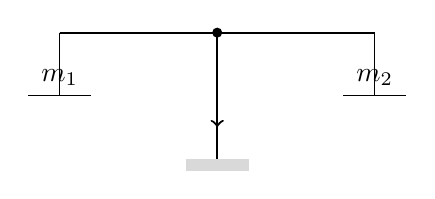
\begin{tikzpicture}[scale=0.8]
        % Base
        \fill[gray!30] (-0.5,0) rectangle (0.5,-0.2);
        \draw[thick] (0,0) -- (0,2); % Asta verticale
        \filldraw (0,2) circle (2pt); % Fulcro
        
        % Braccio orizzontale
        \draw[thick] (-2.5,2) -- (2.5,2);
        
        % Piatti
        \draw (-2.5,2) -- (-2.5,1);
        \draw (-3,1) -- (-2,1); % Piatto sx
        \node[above] at (-2.5,1) {$m_1$};
        
        \draw (2.5,2) -- (2.5,1);
        \draw (2,1) -- (3,1); % Piatto dx
        \node[above] at (2.5,1) {$m_2$};
        
        % Indicatore equilibrio
        \draw[->, thick] (0,1.5) -- (0,0.5);
    \end{tikzpicture}
    \caption{Schema di principio della bilancia a bracci uguali.}
    \label{fig:bilancia_schema}
\end{figure}

\subsection{Massa Inerziale e Gravitazionale}
In realtà, la massa può essere distinta in due diverse tipologie concettuali:
\begin{itemize}
    \item \textbf{Massa Inerziale} ($m_i$): rappresenta la capacità di un corpo di opporsi al moto (resistenza all'accelerazione).
    \item \textbf{Massa Gravitazionale} ($m_g$): rappresenta la capacità di un corpo di attrarre altri corpi (carica gravitazionale).
\end{itemize}

\begin{teorema}{Equivalenza Massa Inerziale e Gravitazionale}
Sebbene concettualmente diverse (\textbf{$m_i$}: resistenza al moto; \textbf{$m_g$}: capacità di attrarre/essere attratti), gli esperimenti di \textbf{Eötvös} hanno dimostrato con altissima precisione che il loro rapporto è costante per tutti i corpi. Nel SI si assume:
\[ m_i = m_g = m \]
\end{teorema}

\begin{osservazione}{Principio di Equivalenza Debole}
Pertanto si può costatare l'uguaglianza numerica tra le due grandezze:
\[ m_i = m_g = m \]
\end{osservazione}

\subsection{La Forza Peso}
La \textbf{Forza Peso} è la forza esercitata dalla Terra su un corpo.
\begin{equation}
    \vec{P} = m \vec{g} \quad \text{con } |\vec{g}| \approx \SI{9.81}{m/s^2}
\end{equation}

L'accelerazione di gravità $\vec{g}$ \textbf{non è costante} su tutta la superficie terrestre. In effetti, essa è una grandezza puntuale e locale che varia in base a:
\begin{enumerate}
    \item \textbf{Rotazione Terrestre}: $\vec{g}$ è maggiore ai poli e minore all'equatore (a causa della forza centrifuga).
    \item \textbf{Geoide}: La Terra è una sfera imperfetta.
    \begin{itemize}
        \item Più in alto $\rightarrow$ $\vec{g}$ diminuisce (lontananza dal centro).
        \item Più in basso $\rightarrow$ $\vec{g}$ aumenta.
    \end{itemize}
    \item \textbf{Disomogeneità Locali}: Presenza di materiali a diversa densità nel sottosuolo.
\end{enumerate}

La misurazione precisa di $\vec{g}$ avviene attraverso particolari pendoli con una risoluzione dell'ordine di $10^{-5}$ (Gravimetria).

\subsection{Differenza tra Massa e Peso}

\begin{figure}[h!]
    \centering
    \begin{tikzpicture}[
        node distance=2cm,
        box/.style={draw, rounded corners, align=center, minimum width=2.5cm, minimum height=1cm, font=\small},
        arrow/.style={->, >=stealth, thick}
    ]
        % Nodo radice
        \node (diff) [box, fill=gray!10] {\textbf{Differenza Massa $\neq$ Peso}};
        
        % Nodi figli
        \node (massa) [box, below left=1cm and 0.2cm of diff, fill=mypen!10] {\textbf{Massa}};
        \node (peso) [box, below right=1cm and 0.2cm of diff, fill=mypen!10] {\textbf{Peso}};
        
        % Caratteristiche Massa
        \node (m_desc) [below=0.2cm of massa, align=center, font=\small] {
            $\bullet$ Grandezza \textbf{Scalare}\\
            $\bullet$ Proprietà \textbf{Intrinseca}
        };
        
        % Caratteristiche Peso
        \node (p_desc) [below=0.2cm of peso, align=center, font=\small] {
            $\bullet$ Grandezza \textbf{Vettoriale}\\
            $\bullet$ Dipendente da $\vec{g}$ e $\vec{a}$
        };
        
        % Frecce
        \draw[arrow] (diff) -- (massa);
        \draw[arrow] (diff) -- (peso);
        
    \end{tikzpicture}
    \caption{Schema delle differenze fondamentali tra Massa e Peso.}
    \label{fig:diff_massa_peso}
\end{figure}

\begin{esercizio}{L'Ascensore e il Peso Apparente}
Un corpo di massa $m$, posto su una bilancia all'interno di un ascensore, è soggetto alla forza peso $\vec{P} = m\vec{g}$ e alla reazione vincolare $\vec{N}$ della bilancia. La bilancia misura la reazione vincolare $\vec{N}$ (il "peso apparente").

Dalla seconda legge della dinamica: $N = m(g + a)$. Analizziamo i casi:
\begin{enumerate}
    \item \textbf{Ascensore fermo ($a=0$)}: $N = mg$. Peso reale.
    \item \textbf{Ascensore accelera verso l'alto ($a > 0$)}: $N = m(g + a) > mg$. Ci sentiamo più pesanti.
    \item \textbf{Ascensore accelera verso il basso ($a < 0$)}: $N = m(g - |a|) < mg$. Ci sentiamo più leggeri.
    \item \textbf{Caduta Libera ($a = -g$)}: $N = 0$. \textbf{Imponderabilità} (assenza di peso).
\end{enumerate}

    \begin{center}
    \begin{tikzpicture}[scale=1.0, >=stealth]
        \tikzset{
            cabin/.style={draw=black!70, thick, rounded corners=3pt, fill=gray!6, minimum width=3.2cm, minimum height=3.8cm},
            person/.style={circle, draw=mypen!60, fill=mypen!25, minimum size=0.7cm, thick},
            fvec/.style={->, line width=1.6pt},
            avec/.style={->, line width=2.2pt, violet}
        }
        % Caso a=0
        \begin{scope}[xshift=0cm]
            \node[cabin] at (0, 1.9) {};
            \node[person] (Hd1) at (0, 1.9) {\scriptsize $m$};
            \draw[fvec, mygreen!80] (Hd1.south) -- ++(0,-1.1) node[right=3pt] {$\vec{P}$};
            \draw[fvec, mypen!80] (Hd1.north) -- ++(0,+0.85) node[right=3pt] {$\vec{N}$};
            \node[below=6pt] at (0,0) {\textbf{$a=0$}};
        \end{scope}
        % Caso a > 0
        \begin{scope}[xshift=5.5cm]
            \node[cabin] at (0, 1.9) {};
            \node[person] (Hd2) at (0, 1.9) {\scriptsize $m$};
            \draw[fvec, mygreen!80]  (Hd2.south) -- ++(0,-1.1) node[right=3pt] {$\vec{P}$};
            \draw[fvec, line width=2.4pt, mypen!80] (Hd2.north) -- ++(0,+1.55) node[right=3pt] {$\vec{N}$};
            \draw[avec] (-2.2, 1.2) -- (-2.2, 2.8) node[above, violet] {$\vec{a}$};
            \node[below=6pt] at (0,0) {\textbf{$a > 0$}};
        \end{scope}
        % Caso a < 0
        \begin{scope}[xshift=11cm]
            \node[cabin] at (0, 1.9) {};
            \node[person] (Hd3) at (0, 1.9) {\scriptsize $m$};
            \draw[fvec, mygreen!80]  (Hd3.south) -- ++(0,-1.1) node[right=3pt] {$\vec{P}$};
            \draw[fvec, mypen!80] (Hd3.north) -- ++(0,+0.45) node[right=3pt] {$\vec{N}$};
            \draw[avec] (-2.2, 2.8) -- (-2.2, 1.2) node[below, violet] {$\vec{a}$};
            \node[below=6pt] at (0,0) {\textbf{$a < 0$}};
        \end{scope}
    \end{tikzpicture}
    \captionof{figure}{Variazione del peso apparente $\vec{N}$ nell'ascensore.}
    \end{center}
\end{esercizio}

\section{Forze di Contatto}
\label{sec:forze_contatto}

Le \textbf{Forze Vincolari (o Normali)} sono forze che uno o più corpi esercitano su un altro limitandone il moto.

\subsection{Equazioni del Vincolo}
Un vincolo impone delle condizioni geometriche alle coordinate del corpo. Ecco i tre casi principali (Fig. \ref{fig:vincoli_rappresentazione}):

\begin{figure}[h!]
    \centering
    % Use minipage for better alignment
    \begin{minipage}{0.31\textwidth}
        \centering
        \textbf{Piano (Tavolo)}
        \vspace{0.2cm}
        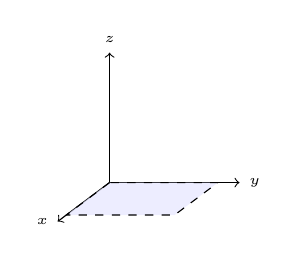
\begin{tikzpicture}[scale=0.55, x={(-0.4cm,-0.3cm)}, y={(1cm,0cm)}, z={(0cm,1cm)}]
            % Assi
            \draw[->] (0,0,0) -- (3,0,0) node[left] {\tiny $x$};
            \draw[->] (0,0,0) -- (0,3,0) node[right] {\tiny $y$};
            \draw[->] (0,0,0) -- (0,0,3) node[above] {\tiny $z$};
            % Piano
            \fill[blue!10, opacity=0.7] (0,0,0) -- (2.5,0,0) -- (2.5,2.5,0) -- (0,2.5,0) -- cycle;
            \draw[dashed] (0,0,0) -- (2.5,0,0) -- (2.5,2.5,0) -- (0,2.5,0) -- cycle;
        \end{tikzpicture}
        \vspace{0.1cm}
        {\scriptsize $z(t) = 0$}
    \end{minipage}
    \hfill
    \begin{minipage}{0.31\textwidth}
        \centering
        \textbf{Circolare}
        \vspace{0.2cm}
        \begin{tikzpicture}[scale=0.55, x={(-0.4cm,-0.3cm)}, y={(1cm,0cm)}, z={(0cm,1cm)}]
            % Assi
            \draw[->] (0,0,0) -- (3,0,0);
            \draw[->] (0,0,0) -- (0,3,0);
            \draw[->] (0,0,0) -- (0,0,3);
            % Cerchio
            \draw[thick, red] (2,0,0) arc (0:90:2);
            \draw[dashed, red] (2,0,0) -- (0,0,0) -- (0,2,0);
            \node[red, right] at (1,0,0) {\tiny $R$};
        \end{tikzpicture}
        \vspace{0.1cm}
        {\scriptsize $x^2 + y^2 = R^2$}
    \end{minipage}
    \hfill
    \begin{minipage}{0.31\textwidth}
        \centering
        \textbf{Piano Inclinato}
        \vspace{0.2cm}
        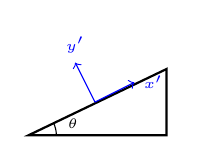
\begin{tikzpicture}[scale=0.7]
            % Cuneo
            \draw[thick] (0,0) -- (2.5,0) -- (2.5,1.2) -- cycle;
            \draw (0.5,0) arc (0:26:0.5);
            \node at (0.8,0.2) {\tiny $\theta$};
            % Sistema ruotato
            \begin{scope}[shift={(1.2, 0.6)}, rotate=26.56]
                \draw[->, blue] (0,0) -- (0.8,0) node[right] {\tiny $x'$};
                \draw[->, blue] (0,0) -- (0,0.8) node[above] {\tiny $y'$};
            \end{scope}
        \end{tikzpicture}
        \vspace{0.1cm}
        {\scriptsize $y'(t) = 0$}
    \end{minipage}
    
    \caption{Rappresentazione grafica delle equazioni dei vincoli per diverse geometrie.}
    \label{fig:vincoli_rappresentazione}
\end{figure}

\begin{osservazione}{La Reazione Vincolare}
Il fatto che sul piano orizzontale statico risulti $\vec{N} + \vec{P} = 0$ (ovvero $\vec{N} = -\vec{P}$) è \textbf{del tutto casuale}. Infatti $|\vec{N}|$ non corrisponde a $|-\vec{P}|$ in un piano inclinato, né in un ascensore accelerato.

$\vec{P} = m\vec{g}$ esiste anche se non ci fosse la $\vec{N}$ del tavolo. Questo perché il $3^{\circ}$ principio non si applica al sistema corpo-tavolo, ma al sistema \textbf{Corpo-Terra}. Il tavolo è solo il vincolo che impedisce il naturale moto dei gravi verso la Terra.
\end{osservazione}

\subsection{Tipologie di Vincoli}

\subsubsection{Cerniere e Tensioni}

\begin{figure}[h!]
    \centering
    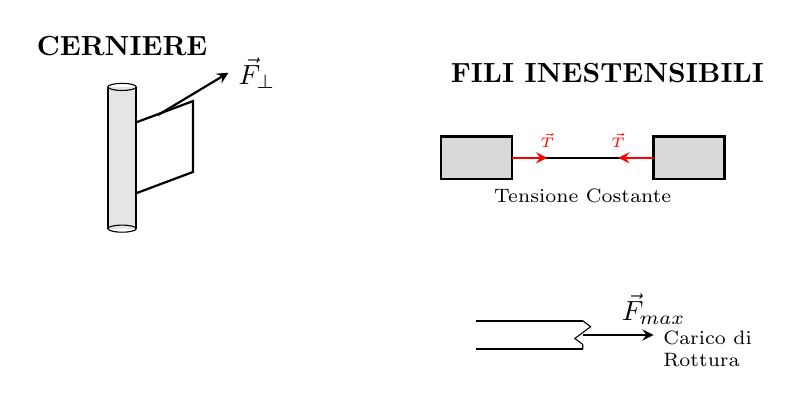
\begin{tikzpicture}[>=stealth, scale=0.9]

        % 1. CERNIERE
        \begin{scope}[xshift=-4cm]
            \node[align=center, anchor=south, font=\bfseries] at (0, 2.3) {CERNIERE};
            % Cilindro/Cerniera
            \fill[gray!20] (-0.2,0) rectangle (0.2,2);
            \draw[thick] (-0.2,0) -- (-0.2,2); \draw[thick] (0.2,0) -- (0.2,2);
            \draw (0,2) ellipse (0.2 and 0.05); \draw (0,0) ellipse (0.2 and 0.05);
            % Staffa
            \draw[thick] (0.2, 1.5) -- (1, 1.8) -- (1, 0.8) -- (0.2, 0.5);
            % Vettore
            \draw[->, thick] (0.5, 1.6) -- (1.5, 2.2) node[right] {$\vec{F}_{\perp}$};
        \end{scope}

        % 2. TENSIONE (BLOCCHI)
        \begin{scope}[xshift=2cm, yshift=1cm]
            \node[anchor=west, font=\bfseries] at (-1.5, 1.2) {FILI INESTENSIBILI};
            \draw[thick, fill=gray!30] (-1.5, -0.3) rectangle (-0.5, 0.3); % Blocco 1
            \draw[thick, fill=gray!30] (1.5, -0.3) rectangle (2.5, 0.3); % Blocco 2
            \draw[thick] (-0.5, 0) -- (1.5, 0); % Filo
            % Vettori Tensione
            \draw[->, thick, red] (-0.5, 0) -- (0, 0) node[above, font=\tiny] {$\vec{T}$};
            \draw[->, thick, red] (1.5, 0) -- (1, 0) node[above, font=\tiny] {$\vec{T}$};
            \node[below, font=\scriptsize] at (0.5, -0.3) {Tensione Costante};
        \end{scope}

        % 3. CARICO DI ROTTURA (FUNE)
        \begin{scope}[xshift=2cm, yshift=-1.5cm]
            % Fune spessa
            \draw[thick] (-1, 0.2) -- (0.5, 0.2); 
            \draw[thick] (-1, -0.2) -- (0.5, -0.2);
            % Rottura
            \draw[decorate, decoration={zigzag, segment length=3mm, amplitude=1mm}] (0.5,0.2) -- (0.5,-0.2);
            
            \draw[->, thick] (0.5, 0) -- (1.5, 0) node[above] {$\vec{F}_{max}$};
            \node[right, font=\scriptsize, align=left] at (1.5, -0.2) {Carico di\\Rottura};
        \end{scope}

    \end{tikzpicture}
    \caption{Esempi di forze vincolari: cerniere che esercitano forze perpendicolari all'asse e fili che trasmettono tensioni.}
    \label{fig:vincoli_tipi}
\end{figure}

\subsubsection{Vincoli Lisci e Scabri}

\begin{itemize}
    \item \textbf{VINCOLO LISCIO}: Esercita solo forze vincolari perpendicolari alla superficie di contatto ($\vec{N}$). Non vi è alcuna forza che si oppone al moto laterale.
    \item \textbf{VINCOLO SCABRO}: Esercita una reazione vincolare $\vec{R}$ che ha due componenti:
    \begin{enumerate}
        \item \textbf{Normale} ($\vec{N}$): perpendicolare alla superficie.
        \item \textbf{Attrito} ($\vec{F}_{att}$): parallela alla superficie e opposta al verso del moto (o dell'imminente moto).
    \end{enumerate}
\end{itemize}

\begin{figure}[h!]
    \centering
    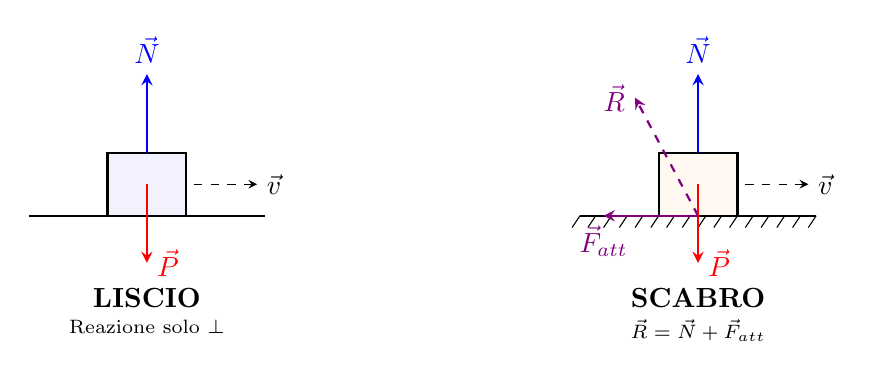
\begin{tikzpicture}[scale=1, >=stealth]
        % --- Liscio ---
        \begin{scope}[xshift=-3.5cm]
            \draw[thick] (-1.5,0) -- (1.5,0);
            \draw[thick, fill=blue!5] (-0.5,0) rectangle (0.5,0.8);
            
            \draw[->, thick, blue] (0,0.8) -- (0,1.8) node[above] {$\vec{N}$};
            \draw[->, thick, red] (0,0.4) -- (0,-0.6) node[right] {$\vec{P}$};
            \draw[->, dashed, black] (0.6,0.4) -- (1.4,0.4) node[right] {$\vec{v}$};
            
            \node[below, font=\bfseries] at (0,-0.8) {LISCIO};
            \node[below, font=\scriptsize] at (0,-1.2) {Reazione solo $\perp$};
        \end{scope}

        % --- Scabro ---
        \begin{scope}[xshift=3.5cm]
            \draw[thick] (-1.5,0) -- (1.5,0);
            \foreach \x in {-1.5,-1.3,...,1.5} \draw (\x,0) -- (\x-0.1,-0.15); % Tratteggio terreno
            \draw[thick, fill=orange!5] (-0.5,0) rectangle (0.5,0.8);
            
            % Reazione Totale R
            \draw[->, thick, violet, dashed] (0,0) -- (-0.8, 1.5) node[left] {$\vec{R}$};
            
            % Componenti
            \draw[->, thick, blue] (0,0.8) -- (0,1.8) node[above] {$\vec{N}$};
            \draw[->, thick, red] (0,0.4) -- (0,-0.6) node[right] {$\vec{P}$};
            \draw[->, thick, violet] (0,0) -- (-1.2,0) node[below] {$\vec{F}_{att}$};
            
            \draw[->, dashed, black] (0.6,0.4) -- (1.4,0.4) node[right] {$\vec{v}$};
            
            \node[below, font=\bfseries] at (0,-0.8) {SCABRO};
            \node[below, font=\scriptsize] at (0,-1.2) {$\vec{R} = \vec{N} + \vec{F}_{att}$};
        \end{scope}
    \end{tikzpicture}
    \caption{Differenza tra vincolo liscio e scabro. Nel vincolo scabro la reazione vincolare $\vec{R}$ non è perpendicolare alla superficie.}
    \label{fig:liscio_vs_scabro}
\end{figure}

Dove $\mu_s$ è il \textbf{Coefficiente di Attrito Statico} (adimensionale), che dipende dalla natura dei materiali e dalla levigatezza delle superfici.

\begin{figure}[h!]
    \centering
    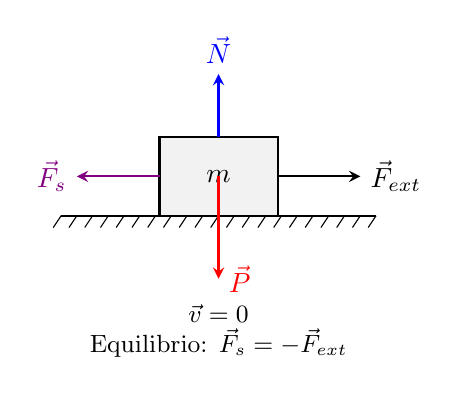
\begin{tikzpicture}[>=stealth, scale=1]
        % Piano
        \draw[thick] (-2,0) -- (2,0);
        \foreach \x in {-2,-1.8,...,2} \draw (\x,0) -- (\x-0.1,-0.15);
        
        % Corpo
        \draw[thick, fill=gray!10] (-0.75,0) rectangle (0.75,1);
        \node at (0,0.5) {$m$};
        
        % Forze
        \draw[->, thick, blue] (0,1) -- (0,1.8) node[above] {$\vec{N}$};
        \draw[->, thick, red] (0,0.5) -- (0,-0.8) node[right] {$\vec{P}$};
        
        \draw[->, thick, black] (0.75,0.5) -- (1.8,0.5) node[right] {$\vec{F}_{ext}$};
        \draw[->, thick, violet] (-0.75,0.5) -- (-1.8,0.5) node[left] {$\vec{F}_s$};
        
        \node[below, align=center, font=\small] at (0,-1) {$\vec{v} = 0$\\Equilibrio: $\vec{F}_s = - \vec{F}_{ext}$};
    \end{tikzpicture}
    \caption{Attrito Statico: si oppone alla forza motrice finché il corpo è fermo.}
\end{figure}

\subsubsection{Attrito Dinamico ($F_d$)}
È la forza parallela alla superficie presente quando il corpo è \textbf{in moto} relativo su una superficie scabra.
Si oppone sempre al versore della velocità istantanea $\hat{v}$.

A differenza dell'attrito statico, l'attrito dinamico ha un modulo (approssimativamente) \textbf{costante} durante il moto, indipendentemente dalla velocità:

\begin{equation}
    |\vec{F}_d| = \mu_d |\vec{N}|
\end{equation}

In forma vettoriale:
\begin{equation}
    \vec{F}_d = - \mu_d |\vec{N}| \hat{v}
\end{equation}

Dove:
\begin{itemize}
    \item $\mu_d$ è il \textbf{Coefficiente di Attrito Dinamico} (solitamente $\mu_d < \mu_s$).
    \item Il segno meno unito al versore $\hat{v}$ indica che il verso di $\vec{F}_d$ è sempre \textbf{opposto} a quello del moto (della velocità e dello spostamento elementare).
    \item \textbf{Nota Bene}: È SBAGLIATO scrivere $\vec{F}_d = -\mu_d \vec{N}$, poiché $\vec{F}_d$ (parallela al piano) e $\vec{N}$ (perpendicolare) sono vettori ortogonali! La relazione vettoriale corretta lega attrito e velocità.
\end{itemize}

\begin{figure}[h!]
    \centering
    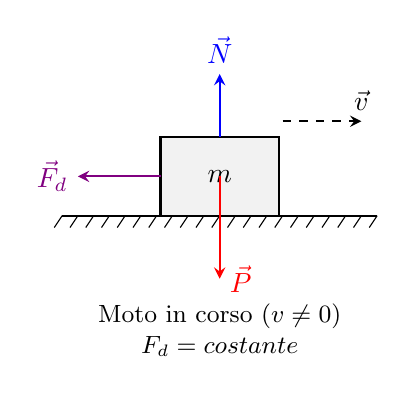
\begin{tikzpicture}[>=stealth, scale=1]
        % Piano
        \draw[thick] (-2,0) -- (2,0);
        \foreach \x in {-2,-1.8,...,2} \draw (\x,0) -- (\x-0.1,-0.15);
        
        % Corpo
        \draw[thick, fill=gray!10] (-0.75,0) rectangle (0.75,1);
        \node at (0,0.5) {$m$};
        
        % Velocità
        \draw[->, dashed, thick, black] (0.8, 1.2) -- (1.8, 1.2) node[above] {$\vec{v}$};
        
        % Forze
        \draw[->, thick, blue] (0,1) -- (0,1.8) node[above] {$\vec{N}$};
        \draw[->, thick, red] (0,0.5) -- (0,-0.8) node[right] {$\vec{P}$};
        
        \draw[->, thick, violet] (-0.75,0.5) -- (-1.8,0.5) node[left] {$\vec{F}_d$};
        
        \node[below, align=center, font=\small] at (0,-1) {Moto in corso ($v \neq 0$)\\$F_d = \text{costante}$};
    \end{tikzpicture}
    \caption{Attrito Dinamico: si oppone alla velocità del corpo.}
    \label{fig:attrito_dinamico}
\end{figure}

\subsubsection{Confronto tra Attriti: Il Caso del Piano Inclinato}
In generale, la forza limite che separa lo stato di \textbf{QUIETE} (in cui agisce l'attrito statico $\vec{F}_s$) dallo stato di \textbf{MOTO} (in cui agisce l'attrito dinamico $\vec{F}_d$) corrisponde alla forza di attrito statico massima ($F_{s,max}$).

Consideriamo il caso generico di un corpo su un \textbf{piano inclinato} di un angolo $\theta$. Ci troviamo nella situazione limite in cui il corpo è sul punto di muoversi (imminente moto), quindi $F_s = F_{s,max} = \mu_s N$.

Scomponiamo le forze lungo gli assi:
\begin{itemize}
    \item Asse $x$ (parallelo al piano, verso il basso): componente parallela del peso $P_{\parallel} = mg \sin\theta$ e forza d'attrito statico $F_s$ (che si oppone allo scivolamento).
    \item Asse $y$ (perpendicolare al piano): reazione vincolare $N$ e componente normale del peso $P_{\perp} = mg \cos\theta$.
\end{itemize}

Il sistema all'equilibrio limite diventa:
\begin{equation}
\begin{cases}
    \sum F_x = m g \sin\theta - F_{s,max} = 0 \\
    \sum F_y = N - m g \cos\theta = 0
\end{cases}
\implies
\begin{cases}
    \mu_s N = m g \sin\theta \\
    N = m g \cos\theta
\end{cases}
\end{equation}

Sostituendo la seconda equazione nella prima:
\[ \mu_s (mg \cos\theta) = mg \sin\theta \]

Semplificando la massa $m$ e l'accelerazione $g$, otteniamo una relazione fondamentale:
\begin{equation}
    \mu_s = \frac{\sin\theta}{\cos\theta} = \tan\theta
\end{equation}

\paragraph{Angolo Critico ($\theta_{max}$)}
Ragionando all'opposto, possiamo calcolare l'angolo massimo di inclinazione $\theta_{max}$ per cui il corpo rimane fermo:
\[ \theta_{max} = \arctan(\mu_s) \]

\begin{itemize}
    \item Finché $\theta < \theta_{max}$: il corpo resta \textbf{fermo} ($F_s < F_{s,max}$).
    \item Quando $\theta > \theta_{max}$: la componente parallela del peso supera l'attrito massimo e il corpo \textbf{scivola}.
\end{itemize}

Geometricamente, questo definisce il cosiddetto \textbf{Cono di Attrito Statico}: se la risultante delle forze di contatto cade all'interno di questo cono di apertura $2\theta_{max}$, il corpo rimane in equilibrio.

\begin{figure}[h!]
    \centering
    \begin{minipage}{0.48\textwidth}
        \centering
        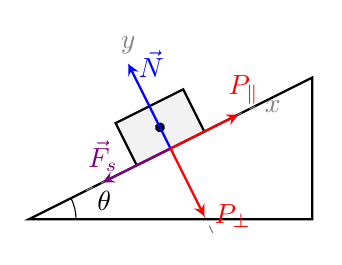
\begin{tikzpicture}[scale=1.2, >=stealth]
            % Piano Inclinato
            \coordinate (A) at (0,0);
            \coordinate (B) at (3,0);
            \coordinate (C) at (3,1.5); % tan(theta) = 0.5 -> theta approx 26.5 deg
            \draw[thick] (A) -- (B) -- (C) -- cycle;
            \draw (0.5,0) arc (0:26.5:0.5);
            \node at (0.8,0.2) {$\theta$};

            % Corpo
            \begin{scope}[shift={(1.5, 0.75)}, rotate=26.56]
                \draw[thick, fill=gray!10] (-0.4, 0) rectangle (0.4, 0.5);
                \fill (0, 0.25) circle (1.5pt); % Centro di massa

                % Sistema di riferimento locale
                \draw[gray, dashed] (-1,0) -- (1,0) node[right] {$x$};
                \draw[gray, dashed] (0,-1) -- (0,1) node[above] {$y$};

                % Forze
                \draw[->, thick, blue] (0, 0) -- (0, 1) node[right] {$\vec{N}$};
                \draw[->, thick, violet] (0, 0) -- (-0.8, 0) node[above] {$\vec{F}_{s}$};
                
                % Peso (non ruotato rispetto alla terra, SCOMPOSTO)
                \draw[->, thick, red] (0, 0) -- (0.8, 0) node[above, xshift=2pt] {$P_{\parallel}$};
                \draw[->, thick, red] (0, 0) -- (0, -0.8) node[right] {$P_{\perp}$};
                
            \end{scope}
            
        \end{tikzpicture}
        \caption{Equilibrio limite su piano inclinato.}
        \label{fig:piano_inclinato_attrito}
    \end{minipage}
    \hfill
    \begin{minipage}{0.48\textwidth}
        \centering
        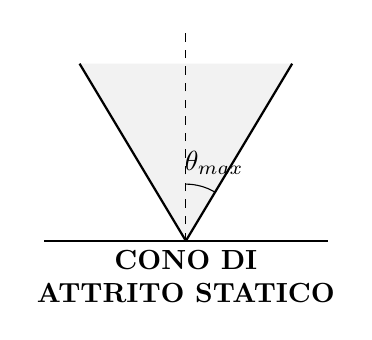
\begin{tikzpicture}[scale=0.9]
            % Piano
            \draw[thick] (-2,0) -- (2,0);
            % Cono
            \fill[gray!10] (0,0) -- (1.5, 2.5) -- (-1.5, 2.5) -- cycle;
            \draw[dashed] (0,0) -- (0,3);
            
            \draw[thick] (0,0) -- (1.5, 2.5);
            \draw[thick] (0,0) -- (-1.5, 2.5);
            
            % Angolo
            \draw (0,0.8) arc (90:59:0.8);
            \node at (0.4, 1.1) {$\theta_{max}$};
            
            \node[align=center, below] at (0,0) {\textbf{CONO DI}\\\textbf{ATTRITO STATICO}};
        \end{tikzpicture}
        \caption{Cono di Attrito.}
        \label{fig:cono_attrito}
    \end{minipage}
\end{figure}

\paragraph{Nota sul piano orizzontale ($\theta = 0$):}
Su un piano orizzontale, in assenza di altre forze esterne, $P_{\parallel} = m g \sin(0) = 0$, quindi la forza di attrito necessaria per l'equilibrio è nulla.
Per misurare $\mu_s$ su un piano orizzontale, bisogna applicare una forza esterna $F_{min}$ finché il corpo non si stacca:
\[ F_{min} = |F_{s,max}| = \mu_s m g \implies \mu_s = \frac{F_{min}}{m g} \]
Dopo lo stacco, se vogliamo mantenere il corpo a velocità costante ($a=0$), dovremo applicare una forza pari all'attrito dinamico: 
\[ F_{motrice} = F_d = \mu_d m g \]
Essendo solitamente $\mu_d < \mu_s$, la forza necessaria per mantenere il moto uniforme è minore di quella necessaria per avviarlo (forza di primo distacco).

\begin{esercizio}{Dinamica del Moto sul Piano Inclinato con Attrito}
Analizziamo il moto di un corpo di massa $m$ su un piano inclinato di un angolo $\theta$.

    \begin{center}
    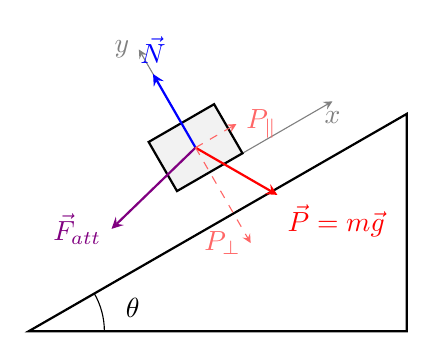
\begin{tikzpicture}[scale=1.2, >=stealth]
        % Piano Inclinato
        \draw[thick] (0,0) -- (4,0) -- (4,2.3) -- cycle;
        \draw (0.8,0) arc (0:30:0.8);
        \node at (1.1, 0.25) {$\theta$};
        
        % Assi ruotati
        \begin{scope}[rotate=30, shift={(2.5, 0.5)}]
             \draw[->, gray] (0,0) -- (1.5,0) node[below] {$x$};
             \draw[->, gray] (0,0) -- (0,1.5) node[left] {$y$};
             
             % Corpo
             \draw[thick, fill=gray!10] (-0.4,0) rectangle (0.4,0.6);
             \coordinate (C) at (0,0.3);
             
             % Forze
             \draw[->, thick, blue] (C) -- (0, 1.2) node[above] {$\vec{N}$};
             \draw[->, thick, violet] (C) -- (-1.2, 0) node[left] {$\vec{F}_{att}$};
             
             % Peso
             \draw[->, thick, red] (C) -- ++(0.5, -0.866) node[below right] {$\vec{P} = m\vec{g}$};
             
             % Scomposizione Peso
             \draw[->, dashed, red!60] (C) -- (0.5, 0.3) node[right] {$P_{\parallel}$};
             \draw[->, dashed, red!60] (C) -- (0, -0.866) node[left] {$P_{\perp}$};
        \end{scope}
    \end{tikzpicture}
    \end{center}

\textbf{Equazioni del moto}:
Proiettando le forze sugli assi $x$ (parallelo al piano) e $y$ (normale):
\begin{itemize}
    \item \textbf{Asse $y$}: $N - mg \cos\theta = 0 \implies N = mg \cos\theta$
    \item \textbf{Asse $x$ (Corpo fermo)}: $mg \sin\theta - F_s = 0 \implies F_s = mg \sin\theta$
    \item \textbf{Asse $x$ (Corpo in moto)}: $mg \sin\theta \mp F_D = ma$
\end{itemize}

\textbf{Accelerazione in discesa}:
\[ a = g(\sin\theta - \mu_D \cos\theta) \]
Velocità finale dopo aver percorso una distanza $L$ partendo da fermo:
\[ v_f = \sqrt{2 L g (\sin\theta - \mu_D \cos\theta)} \]

\textbf{Accelerazione in salita}:
\[ a = g(\sin\theta + \mu_D \cos\theta) \]
Se lanciato con velocità $v_0$, lo spazio $S$ percorso prima di fermarsi è:
\[ S = \frac{v_0^2}{2g(\sin\theta + \mu_D \cos\theta)} \]
\end{esercizio}

\section{Sistemi con Forze di Tensione}
Le forze di tensione si manifestano in presenza di fili o funi tese. Esiste una differenza sostanziale tra \textbf{funi} (con massa non trascurabile) e \textbf{fili} (ideali, con massa trascurabile).

\subsection{Funi e Fili}
Si definisce \textbf{densità lineare di massa} $\mu = \frac{M}{L} [kg/m]$.

\begin{itemize}
    \item \textbf{FUNI}: Considerando un piccolo elemento di corda $\Delta l$ di massa $\Delta m = \mu \Delta l$:
    
    \begin{center}
    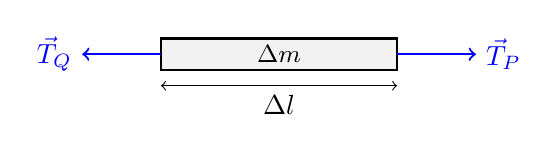
\begin{tikzpicture}
        \draw[thick, fill=gray!10] (0,-0.2) rectangle (3,0.2);
        \draw[->, thick, blue] (3,0) -- (4,0) node[right] {$\vec{T}_P$};
        \draw[->, thick, blue] (0,0) -- (-1,0) node[left] {$\vec{T}_Q$};
        \draw[<->] (0,-0.4) -- (3,-0.4) node[midway, below] {$\Delta l$};
        \node at (1.5, 0) {\small $\Delta m$};
    \end{tikzpicture}
    \end{center}
    
    Se il sistema si muove con accelerazione $\vec{a}$, per il II principio:
    \[ \vec{T}_P - \vec{T}_Q = \Delta m \cdot \vec{a} = (\mu \Delta l) \vec{a} \]
    La tensione non è costante lungo la fune.
    
    \item \textbf{FILI (Ideali)}: Se la massa della fune è trascurabile ($M \approx 0 \implies \mu \approx 0$), allora:
    \[ \vec{T}_P - \vec{T}_Q \approx \vec{0} \implies T_P = T_Q = T \]
    In un filo ideale la tensione è \textbf{costante} in ogni punto.
\end{itemize}

\subsection{Esempio: Sistema Uomo-Cassa}
Consideriamo un uomo che tira una cassa tramite una fune di massa $M$.
\begin{itemize}
    \item Eq. moto fune: $M \vec{a} = \vec{T}_D - \vec{T}_P$
    \item Eq. moto cassa: $m \vec{a} = -\vec{T}_P$
\end{itemize}
Se la fune è un filo ideale ($M=0$), allora $|\vec{F}_{uomo}| = |\vec{T}_P|$, ovvero l'uomo applica la forza direttamente alla cassa.

\subsection{Macchina di Atwood}
La macchina di Atwood consiste in due masse $m_1$ e $m_2$ collegate da un filo ideale che passa sopra una carrucola liscia di massa trascurabile.

\begin{figure}[ht]
    \centering
    \begin{tikzpicture}[scale=0.8]
        % Carrucola
        \draw[thick] (0,0) circle (0.5cm);
        \filldraw (0,0) circle (2pt);
        \draw[thick] (-2,2) -- (2,2);
        \fill[pattern=north east lines] (-2,2) rectangle (2,2.2);
        \draw[thick] (0,2) -- (0,0.5); % Sostegno carrucola
        
        % Filo e masse
        \draw[thick] (-0.5,0) -- (-0.5,-2);
        \draw[thick] (0.5,0) -- (0.5,-3);
        
        \draw[fill=gray!20] (-0.9,-2) rectangle (-0.1,-2.8) node[midway] {$m_1$};
        \draw[fill=gray!20] (0.1,-3) rectangle (0.9,-3.8) node[midway] {$m_2$};
        
        % Forze su m1
        \draw[->, thick, blue] (-0.5,-2) -- (-0.5,-1) node[left] {$\vec{T}$};
        \draw[->, thick, red] (-0.5,-2.4) -- (-0.5,-3.4) node[left] {$m_1\vec{g}$};
        
        % Forze su m2
        \draw[->, thick, blue] (0.5,-3) -- (0.5,-2) node[right] {$\vec{T}$};
        \draw[->, thick, red] (0.5,-3.4) -- (0.5,-4.4) node[right] {$m_2\vec{g}$};
        
        % Assi
        \draw[->, dashed, gray] (1.5, -4) -- (1.5, 0) node[above] {$y$};
    \end{tikzpicture}
    \caption{Schema della Macchina di Atwood.}
\end{figure}

Assumendo $m_1 > m_2$, impostiamo il sistema delle equazioni del moto:
\[
\begin{cases}
    m_1 g - T = m_1 a \\
    T - m_2 g = m_2 a
\end{cases}
\]
Sommando le due equazioni eliminiamo la tensione $T$:
\[ (m_1 - m_2)g = (m_1 + m_2)a \implies \boxed{a = g \frac{m_1 - m_2}{m_1 + m_2}} \]
Sostituendo $a$ in una delle equazioni, troviamo la tensione del filo:
\[ \boxed{T = \frac{2 m_1 m_2}{m_1 + m_2} g} \]

\section{Forze di Attrito Viscoso}
L'attrito viscoso si manifesta quando un corpo solido si muove all'interno di un \textbf{fluido} (liquido o gas). Si tratta di forze frenanti che dipendono dalla velocità del corpo.

\subsection{Legge Empirica e Regimi di Velocità}
In generale, la forza di attrito viscoso può essere espressa come:
\[ \vec{F}_v = -\vec{v} \cdot f(v) \]
Espandendo $f(v)$ in serie di potenze: $f(v) = \alpha + \beta v + \gamma v^2 + \dots$
\begin{itemize}
    \item \textbf{Regime di basse velocità}: $f(v) \approx \alpha$ (costante). La forza è proporzionale alla velocità: $\vec{F}_v = -\alpha \vec{v}$.
    \item \textbf{Regime di alte velocità}: La dipendenza diventa quadratica: $\vec{F}_v \approx -\gamma v^2 \hat{v}$.
\end{itemize}

Per una sfera di raggio $r$, il coefficiente $\alpha$ è dato dalla \textbf{Legge di Stokes}:
\[ \alpha = 6 \pi \eta r \]
dove $\eta$ è la viscosità del mezzo.

\subsection{Equazione del Moto e Velocità Limite}
Se applichiamo una forza costante $\vec{F}$ (es. la gravità) a un corpo in un mezzo viscoso:
\[ m \frac{dv}{dt} = F - \alpha v \implies \frac{dv}{dt} = \frac{F}{m} - \frac{\alpha}{m} v \]
Questa è un'equazione differenziale del I ordine non omogenea. La soluzione è:
\[ v(t) = \frac{F}{\alpha} + \left( v_0 - \frac{F}{\alpha} \right) e^{-t/\tau} \]
dove $\tau = \frac{m}{\alpha}$ è la \textbf{costante di tempo} del sistema.

\paragraph{Velocità di Saturazione (Limite):}
Per $t \to \infty$, il termine esponenziale decade e la velocità tende asintoticamente a un valore costante:
\begin{equation}
    v_L = \lim_{t \to \infty} v(t) = \frac{F}{\alpha}
\end{equation}
In questo stato la forza viscosa bilancia esattamente la forza applicata ($a=0$).

\begin{figure}[ht]
    \centering
    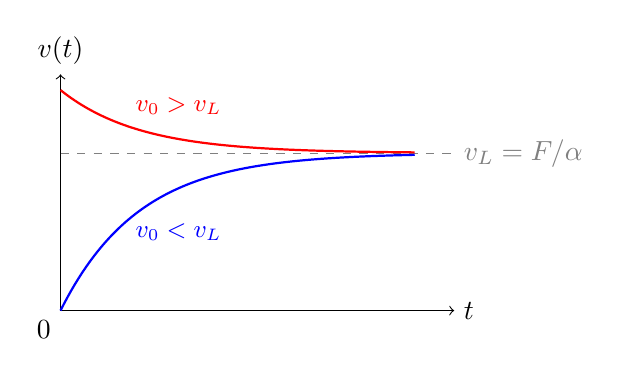
\begin{tikzpicture}
        \draw[->] (0,0) -- (5,0) node[right] {$t$};
        \draw[->] (0,0) -- (0,3) node[above] {$v(t)$};
        
        \draw[dashed, gray] (0,2) -- (5,2) node[right] {$v_L = F/\alpha$};
        
        % Caso v0 < vL
        \draw[thick, blue] plot[domain=0:4.5, samples=100] (\x, {2*(1 - exp(-\x))});
        \node[blue] at (1.5,1) {\small $v_0 < v_L$};
        
        % Caso v0 > vL
        \draw[thick, red] plot[domain=0:4.5, samples=100] (\x, {2 + 0.8*exp(-\x)});
        \node[red] at (1.5,2.6) {\small $v_0 > v_L$};
        
        \node[below left] at (0,0) {$0$};
    \end{tikzpicture}
    \caption{Andamento della velocità verso il valore di saturazione $v_L$.}
\end{figure}

\subsection{Calcolo dello Spazio Percorso}
Consideriamo il caso in cui $F=0$ (corpo lanciato con $v_0$ che viene frenato solo dal fluido):
\[ v(t) = v_0 e^{-t/\tau} \]
Integrando per trovare la posizione $x(t)$:
\[ x(t) = \int_0^t v(t') dt' = \int_0^t v_0 e^{-t'/\tau} dt' = v_0 \tau \left( 1 - e^{-t/\tau} \right) \]
Il corpo percorre una distanza finita prima di fermarsi idealmente (per $t \to \infty$):
\begin{equation}
    \Delta x_{total} = v_0 \tau = \frac{m v_0}{\alpha}
\end{equation}
\subsection{Analisi per Tempi Brevi (\texorpdfstring{$t \ll \tau$}{t << tau})}
Per tempi molto piccoli rispetto alla costante di tempo, possiamo approssimare l'esponenziale con lo sviluppo di Taylor al primo ordine: $e^{-t/\tau} \approx 1 - \frac{t}{\tau}$.
Sostituendo nella legge oraria della velocità:
\[ v(t) = \frac{F}{\alpha} + \left( v_0 - \frac{F}{\alpha} \right) \left( 1 - \frac{t}{\tau} \right) = \frac{F}{\alpha} + v_0 - \frac{F}{\alpha} - v_0\frac{t}{\tau} + \frac{F}{\alpha}\frac{t}{\tau} \]
Dunque:
\begin{equation}
    v(t) \approx v_0 + \left( \frac{F}{\alpha} - v_0 \right) \frac{t}{\tau}
\end{equation}
Questa espressione mostra che per tempi brevi la velocità varia linearmente, come in un moto uniformemente accelerato con accelerazione $a = \frac{F - \alpha v_0}{m}$.

\begin{tcolorbox}[colback=blue!5!white,colframe=blue!75!black,title=\textbf{Effetti della Forza sulla Velocità}]
Le modalità con cui una forza modifica il moto dipendono dalla sua orientazione rispetto al vettore velocità $\vec{v}_0$ istantaneo:
\begin{enumerate}
    \item \textbf{Forza Parallela} ($\vec{F} \parallel \vec{v}_0$): La forza modifica solo il \textbf{modulo} della velocità, non la sua direzione (moto unidimensionale).
    \item \textbf{Forza Perpendicolare} ($\vec{F} \perp \vec{v}_0$): La forza modifica solo la \textbf{direzione} della velocità, mantenendo il modulo costante (es. moto circolare uniforme).
\end{enumerate}
\end{tcolorbox}

\chapter{Lavoro ed Energia}
\section{Definizione di Lavoro}
L'attrito statico è essenziale affinché un veicolo o un uomo/animale possa spostarsi, poiché permette di sfruttare l'aderenza del piano. Tuttavia, da solo non basta; senza una "forza interna" da parte dell'uomo (muscoli) il movimento non potrebbe avvenire.

\textbf{LAVORO ($L$)}: Quando un punto materiale subisce uno spostamento sotto l'azione di una forza, si dice che quest'ultima compie un lavoro sul punto. 
Il lavoro può essere prodotto da una forza:
\begin{itemize}
    \item \textbf{UNIFORME}: Indipendente dalla posizione.
    \item \textbf{VARIA}: Dipendente dalla posizione.
\end{itemize}

\subsection{Caso di Forza Uniforme}
Il lavoro $L$ compiuto da una forza costante $\vec{F}$ durante uno spostamento rettilineo $\vec{s}$ è definito come il prodotto scalare:
\begin{equation}
    L = \vec{F} \cdot \vec{s} = F \cdot s \cdot \cos\theta
\end{equation}

Si distinguono tre casi fondamentali:
\begin{itemize}
    \item $L > 0$ se $0 \leq \theta < \pi/2$: \textbf{LAVORO MOTORE}.
    \item $L < 0$ se $\pi/2 < \theta \leq \pi$: \textbf{LAVORO RESISTENTE (DISSIPATIVO)}.
    \item $L = 0$ se $\theta = \pi/2$: La forza è perpendicolare allo spostamento ($\vec{F} \perp \vec{s}$).
\end{itemize}

\subsection{Caso di Forza Varia}
Per una forza che varia lungo la traiettoria $\gamma$, definiamo il lavoro infinitesimo $dL$ per uno spostamento $d\vec{s}$:
\begin{equation}
    dL = \vec{F} \cdot d\vec{s} = F \cdot ds \cdot \cos\theta
\end{equation}
Il lavoro totale è dato dall'integrale di linea lungo la curva $\gamma$:
\begin{equation}
    L^{(\gamma)} = \int_{R_{in}}^{R_F} \vec{F} \cdot d\vec{s} = \sum_{i=1}^n \Delta L_i \quad \text{per } n \to \infty
\end{equation}

In coordinate cartesiane:
\begin{equation}
    L^{(\gamma)} = \int_{R_{in}}^{R_F} (F_x dx + F_y dy + F_z dz) = L_x + L_y + L_z
\end{equation}
In caso unidimensionale lungo $x$: $L = \int_{x_{in}}^{x_F} F_x dx$, dove $F_x = F \cos\theta$.

\textbf{Unità di misura}: $[L] = [F] \cdot [s] = \text{Newton} \cdot \text{metro} = \text{Joule (J)}$.
$1\text{ J} = 1\text{ kg} \cdot \text{m}^2/\text{s}^2 = 1\text{ N} \cdot \text{m}$.

\section{Lavoro della Forza Peso}
La forza peso è $\vec{P} = m\vec{g} = mg(-\hat{y})$. Il lavoro compiuto dalla forza peso per uno spostamento da $\vec{R}_{in}$ a $\vec{R}_F$ su una traiettoria $\gamma$ è:
\begin{equation}
    L_P^{(\gamma)} = \int_{R_{in}}^{R_F} m\vec{g} \cdot d\vec{s} = m\vec{g} \cdot (\vec{R}_F - \vec{R}_{in}) = m g (y_{in} - y_F) = -mg\Delta h
\end{equation}
Notiamo che $\Delta h = y_F - y_{in}$ deve essere considerato con il suo segno. 
$L_P$ dipende solo da $\Delta h$, poiché $m$ e $g$ (vicino al suolo) rimangono costanti. In particolare:
\begin{itemize}
    \item $L_P > 0$ se $\Delta h < 0$: il corpo scende, $y_F < y_{in}$.
    \item $L_P < 0$ se $\Delta h > 0$: il corpo sale, $y_F > y_{in}$.
\end{itemize}
$\Delta h$ identifica lo \textbf{spostamento globale} lungo la verticale, non lo spazio effettivo percorso seguendo $\gamma$. Infatti $L_P$ non dipende dal percorso seguito ($L_{Pa} = L_{Pb}$).

\begin{figure}[ht]
    \centering
    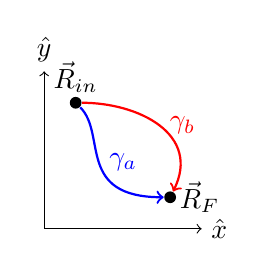
\begin{tikzpicture}[scale=0.8]
        \draw[->] (0,0) -- (0,2.5) node[above] {$\hat{y}$};
        \draw[->] (0,0) -- (2.5,0) node[right] {$\hat{x}$};
        \node at (0.5,2) (A) [circle, fill, inner sep=1.5pt] {};
        \node at (2,0.5) (B) [circle, fill, inner sep=1.5pt] {};
        \draw[->, thick, blue] (A) .. controls (1,1.5) and (0.5,0.5) .. (B) node[midway, right] {$\gamma_a$};
        \draw[->, thick, red] (A) .. controls (1.5,2) and (2.5,1.5) .. (B) node[midway, right] {$\gamma_b$};
        \node[above] at (A) {$\vec{R}_{in}$};
        \node[right] at (B) {$\vec{R}_F$};
    \end{tikzpicture}
    \caption{Indipendenza del lavoro della forza peso dal cammino.}
\end{figure}

\subsection{Esempi di calcolo della velocità finale}
Vediamo come calcolare $v_f$ o $v_0$ in vari scenari:
\begin{enumerate}
    \item \textbf{Caduta libera}: Partendo da fermo ($v_{in}=0$), $v_f = \sqrt{2gh}$.
    \item \textbf{Lancio verso l'alto}: Per raggiungere quota $h$ con $v_f=0$, serve $v_0 = \sqrt{2gh}$.
    \item \textbf{Relazione tra $v^2$ ed $h$}: Come visto dagli esempi, $h = \frac{v^2}{2g}$ e $v^2 = 2gh$. Moltiplicando per $m/2$:
    \begin{equation}
        mgh = \frac{1}{2} m v^2
    \end{equation}
    Dove $\frac{1}{2}mv^2 = E_c$ è l'\textbf{Energia Cinetica} di un punto di massa $m$.
\end{enumerate}

\section{Teorema delle Forze Vive (Lavoro-Energia)}
Si definisce \textbf{Energia Cinetica} ($K$ o $E_c$) di un punto materiale:
\begin{equation}
    K = \frac{1}{2} m v^2
\end{equation}
Relazione fondamentale: $mgh = \frac{1}{2} m v^2 \implies v = \sqrt{2gh}$.

\begin{tcolorbox}[colback=green!5!white,colframe=green!75!black,title=\textbf{Teorema delle Forze Vive}]
Il lavoro compiuto dalla risultante delle forze agenti su un punto materiale è pari alla variazione della sua energia cinetica:
\begin{equation}
    L = \Delta K = K_F - K_{in}
\end{equation}
\end{tcolorbox}

\textit{Dimostrazione}:
\[ L = \int \vec{F} \cdot d\vec{s} = \int m \frac{d\vec{v}}{dt} \cdot \vec{v} dt = \int m \left( \frac{1}{2} \frac{d v^2}{dt} \right) dt = \left[ \frac{1}{2} m v^2 \right]_{in}^F \]

\section{Caso del Pendolo Semplice}
Consideriamo una massa $m$ appesa a un filo di lunghezza $R$. Indicando con $\phi$ l'angolo tra il filo e la verticale (positivo a destra):
\begin{equation}
    m\vec{a} = m\vec{g} + \vec{T} \implies m(\vec{a}_t + \vec{a}_n) = m\vec{g} + \vec{T}
\end{equation}
L'accelerazione in componenti polari ($R$ costante) è:
$\vec{a} = -R\dot{\phi}^2 \hat{n} + R\ddot{\phi} \hat{\tau}$. 
Scriviamo le equazioni del moto per $\hat{\tau}$ ed $\hat{n}$:
\begin{equation}
    \begin{cases}
        \hat{\tau}: m R \ddot{\phi} = -mg \sin\phi \implies \ddot{\phi} = -\frac{g}{R} \sin\phi \\
        \hat{n}: m \frac{v^2}{R} = T - mg \cos\phi \implies T = m \frac{v^2}{R} + mg \cos\phi
    \end{cases}
\end{equation}
Il punto $\phi = 0$ è detto \textbf{centro di oscillazione}.

\subsection{Analisi della Tensione e delle Piccole Oscillazioni}
Per la componente normale, deve essere $T \geq 0$ affinché il filo rimanga teso, altrimenti il corpo cadrebbe. Questo implica $v^2 \geq -R g \cos\phi$. Questo è sempre vero se $-\pi/2 \leq \phi \leq \pi/2$.

\textbf{Piccole oscillazioni}: Per $\phi \ll 1$, usiamo $\sin\phi \approx \phi$. L'equazione diventa $\ddot{\phi} + \frac{g}{R} \phi = 0$.
Definiamo $\omega_0^2 = \frac{g}{R}$, dove $\omega_0$ è la \textbf{pulsazione} (costante).
La soluzione è $\phi(t) = A \cos(\omega_0 t) + B \sin(\omega_0 t)$.
Se il pendolo parte da $\phi_0$ con velocità nulla ($\dot{\phi}=0$):
\begin{equation}
    \phi(t) = \phi_0 \cos(\omega_0 t)
\end{equation}
I punti $\phi = \pm \phi_0$ sono i \textbf{punti di inversione} del moto, dove la velocità $\dot{\phi}(t)$ cambia verso dopo essersi annullata e l'accelerazione $\ddot{\phi}(t)$ è massima e opposta allo spostamento ($\ddot{\phi} \propto -\phi$).

\begin{figure}[ht]
    \centering
    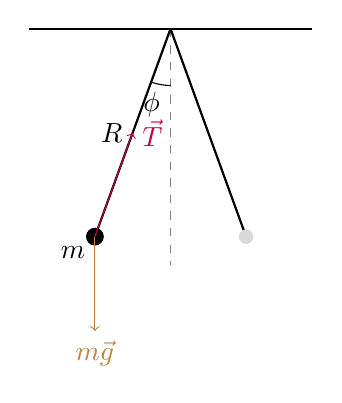
\begin{tikzpicture}[scale=1.2]
        \draw[thick] (-1.5,0) -- (1.5,0);
        \draw[dashed, gray] (0,0) -- (0,-2.5);
        \draw[thick] (0,0) -- (-0.8,-2.2) node[midway, left] {$R$};
        \filldraw (-0.8,-2.2) circle (2.5pt) node[below left] {$m$};
        \draw[thick] (0,0) -- (0.8,-2.2);
        \filldraw[gray!30] (0.8,-2.2) circle (2pt);
        \draw (0,-0.6) arc (-90:-110:0.6);
        \node at (-0.2,-0.8) {$\phi$};
        \draw[->, brown] (-0.8,-2.2) -- (-0.8,-3.2) node[below] {$m\vec{g}$};
        \draw[->, purple] (-0.8,-2.2) -- (-0.4,-1.1) node[right] {$\vec{T}$};
    \end{tikzpicture}
    \caption{Diagramma del pendolo semplice e forze agenti.}
\end{figure}

\section{Forze Elastiche}
L'elasticità è la capacità di tornare allo stato di equilibrio dopo una deformazione. La \textbf{Legge di Hooke} recita: $\vec{F}_{el} = -k \Delta \vec{R}$.
In un piano senza attrito, il moto è descritto da $m \ddot{x} = -k(x - x_0)$, da cui $\ddot{x} + \frac{k}{m}(x - x_0) = 0$.
Questa è un'equazione differenziale di II ordine lineare a coefficienti costanti non omogenea (ma riconducibile a omogenea spostando l'origine). La soluzione è:
\begin{equation}
    x(t) = x_0 + A \cos(\omega_0 t) + B \sin(\omega_0 t) \quad \text{con } \omega_0 = \sqrt{k/m}
\end{equation}

\subsection{Caso della Molla con Forza Costante}
Se la molla è verticale (soggetta a gravità), l'equazione del moto è $m \ddot{x} = mg - k (x - x_0)$.
Ricidendo l'equilibrio ($\ddot{x}=0$), troviamo il punto di equilibrio statico:
$x_{eq} = x_0 + \frac{mg}{k}$.
L'equazione diventa $\ddot{x} = -\frac{k}{m} (x - x_{eq})$.
La soluzione generale per il problema di Cauchy con condizioni iniziali a $t=0$ è:
\begin{equation}
    x(t) = x_{eq} + (x(0) - x_{eq}) \cos(\omega_0 t) + \frac{v(0)}{\omega_0} \sin(\omega_0 t)
\end{equation}
Per risolvere la situazione particolare dobbiamo considerare una situazione specifica (come quella di equilibrio) mentre per l'intera soluzione dobbiamo sfruttare le condizioni iniziali (\textbf{Teorema di Cauchy}).

\begin{definizione}{Energia Potenziale}
Si definisce \textbf{Energia Potenziale} ($U$) la capacità di un sistema di compiere lavoro in virtù della sua configurazione o posizione. La relazione fondamentale tra una forza conservativa e l'energia potenziale associata è:
\begin{equation}
    \vec{F} = -\nabla U
\end{equation}
\end{definizione}

\subsection{Relazione Differenziale e Gradiente}
Considerando un moto unidimensionale lungo l'asse $x$, vogliamo ricavare $F_x(x)$ conoscendo $U(x)$. Partendo dalla definizione di $\Delta U$ per uno spostamento da $x_0$ a $x$:
\begin{equation}
    U(x) - U(x_0) = -\int_{x_0}^x F_{x'}(x') dx'
\end{equation}
Derivando entrambi i membri rispetto a $x$ e applicando il \textbf{Teorema Fondamentale del Calcolo Integrale}:
\begin{equation}
    \frac{d}{dx} [U(x) - U(x_0)] = \frac{d}{dx} \left[ -\int_{x_0}^x F_{x'} dx' \right] \implies \frac{dU}{dx} = -F_x(x)
\end{equation}
Pertanto: $\boxed{F_x(x) = -\frac{dU}{dx}}$. In tre dimensioni, considerando le variazioni lungo ogni asse ($x, y, z$):
\begin{equation}
    F_x = -\frac{\partial U}{\partial x}; \quad F_y = -\frac{\partial U}{\partial y}; \quad F_z = -\frac{\partial U}{\partial z}
\end{equation}
Queste componenti possono essere riunite dal concetto di \textbf{Gradiente} ($\nabla$):
\begin{equation}
    \vec{F} = -\nabla U = -\text{grad } U = -\left( \frac{\partial U}{\partial x} \hat{x} + \frac{\partial U}{\partial y} \hat{y} + \frac{\partial U}{\partial z} \hat{z} \right)
\end{equation}

\subsection{Superfici Equipotenziali}
Una \textbf{superficie equipotenziale} è l'insieme dei punti dello spazio in cui l'energia potenziale assume lo stesso valore ($U(x,y,z) = \text{cost}$). 
Poiché su tale superficie $\Delta U = 0$, il lavoro compiuto dalla forza per spostamenti tangenti alla superficie è nullo. Ne consegue che:
\begin{itemize}
    \item La forza $\vec{F}$ è sempre \textbf{perpendicolare} alle superfici equipotenziali.
    \item La forza punta nella direzione di massima decrescita di $U$.
\end{itemize}

\begin{center}
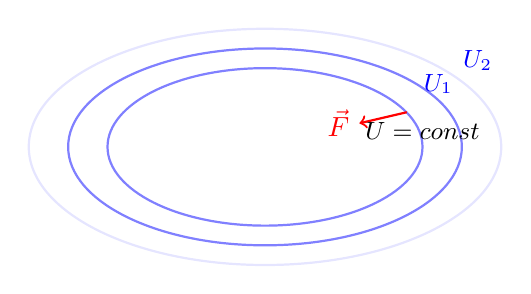
\begin{tikzpicture}
    % Surface lines
    \draw[thick, blue!50] (0,0) ellipse (2cm and 1cm);
    \draw[thick, blue!50] (0,0) ellipse (2.5cm and 1.25cm);
    \draw[thick, blue!10] (0,0) ellipse (3cm and 1.5cm);
    \node[blue] at (2.2,0.8) {\small $U_1$};
    \node[blue] at (2.7,1.1) {\small $U_2$};
    
    % Force vector
    \draw[->, thick, red] (1.8,0.44) -- (1.2,0.3) node[left] {$\vec{F}$};
    \node at (2,0.2) {\small $U = \text{const}$};
\end{tikzpicture}
\end{center}

\subsection{Punti di Equilibrio e Buche di Potenziale}
L'analisi dell'andamento di $U(x)$ permette di identificare i punti di equilibrio ($F_x = -dU/dx = 0$):
\begin{enumerate}
    \item \textbf{Equilibrio Stabile}: Corrisponde a un \textbf{minimo} di $U$. Una piccola perturbazione genera una forza di richiamo verso il punto di equilibrio.
    \item \textbf{Equilibrio Instabile}: Corrisponde a un \textbf{massimo} di $U$. Una perturbazione allontana definitivamente il corpo.
    \item \textbf{Equilibrio Indifferente}: Corrisponde a una regione dove $U$ è costante.
\end{enumerate}

\begin{center}
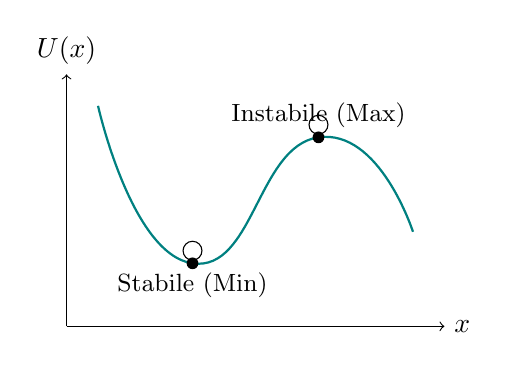
\begin{tikzpicture}[scale=0.8]
    \draw[->] (0,0) -- (6,0) node[right] {$x$};
    \draw[->] (0,0) -- (0,4) node[above] {$U(x)$};
    \draw[thick, teal] plot [smooth, tension=1] coordinates { (0.5,3.5) (2,1) (4,3) (5.5,1.5)};
    
    \node at (2,1) [circle, fill, inner sep=1.5pt] {};
    \node[below] at (2,1) {\small Stabile (Min)};
    \node at (4,3) [circle, fill, inner sep=1.5pt] {};
    \node[above] at (4,3) {\small Instabile (Max)};
    
    % Ball illustrations
    \draw (2,1.2) circle (0.15);
    \draw (4,3.2) circle (0.15);
\end{tikzpicture}
\end{center}

\section{Campi di Forza ed Energia Meccanica}
Un \textbf{Campo} è l'insieme dei valori che una grandezza fisica assume in certe regioni dello spazio. Le forze conservative generano un campo conservativo dove la forza dipende dalla posizione del corpo.
Unendo i punti di applicazione delle forze si ottiene un \textbf{inviluppo} che prende il nome di \textbf{linea di forza} o di campo, a cui $\vec{F}$ è tangente.
\textbf{Proprietà delle linee di forza}:
\begin{enumerate}[label=\alph*)]
    \item Non possono incrociarsi.
    \item Non possono essere chiuse se il campo è conservativo (altrimenti $L = \oint \vec{F} \cdot d\vec{s} \neq 0$).
\end{enumerate}

\subsection{Energia Meccanica}
L'unione dell'energia cinetica $K$ e potenziale $U$ definisce l'\textbf{Energia Meccanica} ($E_{mecc}$):
\begin{equation}
    E_{mecc} = K + U = \frac{1}{2}mv^2 + U(\vec{r}) = \frac{p^2}{2m} + U(\vec{r})
\end{equation}

Dato che in presenza di sole forze conservative ($F_{con}$) l'energia non viene persa, mentre in presenza di forze non conservative ($F_{diss}$) sì, capiamo che la variazione $\Delta E_{mecc}$ è dovuta esclusivamente alle forze dissipative.

\begin{teorema}{Teorema delle Forze Vive (Energia Meccanica)}
Il lavoro totale è la somma del lavoro delle forze conservative e dissipative. $\Delta K + \Delta U = L_{diss}$, ovvero:
\[ \Delta E_{mecc} = L_{diss} \]
\end{teorema}

\subsection{Principio di Conservazione dell'Energia}
"L'energia non si crea né si distrugge, ma si trasforma da una forma all'altra":
\begin{itemize}
    \item Le forze conservative trasformano $K$ in $U$ e viceversa.
    \item Le forze dissipative trasformano $E_{mecc}$ in calore, luce, ecc.
\end{itemize}

\subsection{Teorema della Conservazione dell'Energia Meccanica}
In presenza di sole forze conservative, l'energia meccanica del sistema resta costante durante il moto:
\begin{equation}
    \Delta E_{mecc} = 0 \implies K_i + U_i = K_f + U_f \implies \Delta K = -\Delta U
\end{equation}

\subsection{Regioni Accessibili al Moto (1-D)}
Nei moti 1-D lungo $x$, la conservazione dell'energia implica $E_0 = \frac{1}{2}m\dot{x}^2 + U(x)$. Poiché $K \ge 0$, il moto è possibile solo nelle regioni dove $E_0 \ge U(x)$:
\begin{itemize}
    \item \textbf{Punti di inversione}: $\dot{x} = 0 \implies E_0 = U(x)$.
    \item \textbf{Regioni di moto}: $\dot{x} \neq 0 \implies E_0 > U(x)$.
    \item \textbf{Regioni proibite}: $E_0 < U(x)$ (richiederebbero $K < 0$, impossibile).
\end{itemize}

\begin{center}
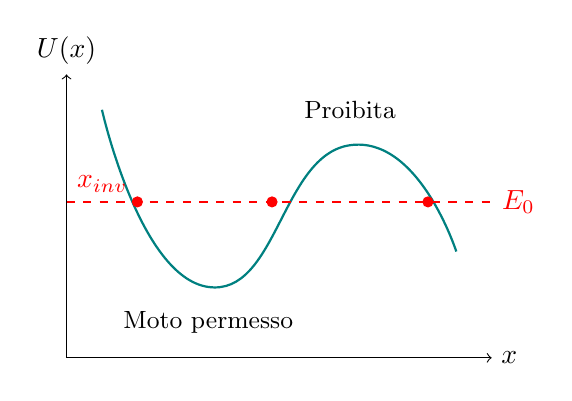
\begin{tikzpicture}[scale=0.9]
    \draw[->] (0,0) -- (6,0) node[right] {$x$};
    \draw[->] (0,0) -- (0,4) node[above] {$U(x)$};
    \draw[thick, teal] plot [smooth, tension=1] coordinates { (0.5,3.5) (2,1) (4,3) (5.5,1.5)};
    
    % Energy level
    \draw[dashed, red, thick] (0,2.2) -- (6,2.2) node[right] {$E_0$};
    
    % Intersection points
    \filldraw[red] (1,2.2) circle (2pt) node[above left] {$x_{inv}$};
    \filldraw[red] (2.9,2.2) circle (2pt);
    \filldraw[red] (5.1,2.2) circle (2pt);
    
    \node at (2,0.5) {\small Moto permesso};
    \node at (4,3.5) {\small Proibita};
\end{tikzpicture}
\end{center}

\section{Dinamica dei Sistemi di Punti Materiali}
Un \textbf{sistema materiale} è un insieme di $N$ punti materiali. Può essere:
\begin{itemize}
    \item \textbf{Discreto}: Punti separati con masse $m_i$.
    \item \textbf{Continuo}: Distribuzione continua di massa con densità $\rho$.
\end{itemize}

\begin{definizione}{Centro di Massa (CM)}
Il centro di massa è il punto in cui immaginiamo concentrata tutta la massa del sistema.
\begin{itemize}
    \item \textbf{Sistema Discreto}: $\vec{R}_{CM} = \frac{\sum m_i \vec{r}_i}{M}$ con $M = \sum m_i$.
    \item \textbf{Sistema Continuo}: $\vec{R}_{CM} = \frac{1}{M} \int \vec{r} dm$, dove $dm = \rho dV$.
\end{itemize}
\end{definizione}

\subsection{Sistema di Riferimento del Centro di Massa}
Il CM può essere usato come origine di un sistema di riferimento rispetto al quale i punti si esprimono con \textbf{coordinate relative} $\vec{r}_i'$:
\begin{equation}
     S \to S' : \vec{r}_i' = \vec{r}_i - \vec{R}_{CM} \iff \vec{r}_i = \vec{r}_i' + \vec{R}_{CM}
\end{equation}
Rispetto a questo sistema, le coordinate del CM sono banalmente $(0,0,0)$. Una proprietà fondamentale è che la sommatoria del momento del primo ordine rispetto al CM è nulla:
\begin{equation}
    \sum m_i \vec{r}_i' = \sum m_i (\vec{r}_i - \vec{R}_{CM}) = \underbrace{\sum m_i \vec{r}_i}_{M \vec{R}_{CM}} - \underbrace{\sum m_i}_{M} \vec{R}_{CM} = \vec{0}
\end{equation}

\subsection{Grandezze Cinetiche del CM}
Seguendo la stessa logica di trasformazione delle coordinate, definiamo le grandezze derivate:
\begin{itemize}
    \item \textbf{Velocità}: $\vec{V}_{CM} = \frac{d\vec{R}_{CM}}{dt} = \frac{1}{M} \sum m_i \vec{v}_i$
    \item \textbf{Quantità di Moto}: $\vec{P}_{tot} = M \vec{V}_{CM} = \sum m_i \vec{v}_i$
    \item \textbf{Accelerazione}: $\vec{A}_{CM} = \frac{d\vec{V}_{CM}}{dt} = \frac{1}{M} \sum m_i \vec{a}_i$
\end{itemize}
Si noti che $\vec{v}_i = \vec{v}_i' + \vec{V}_{CM}$ e $\vec{a}_i = \vec{a}_i' + \vec{A}_{CM}$.

\begin{teorema}{Prima Equazione Cardinale}
Per ogni punto del sistema vale $\vec{F}_i^{ext} + \vec{F}_i^{int} = m_i \vec{a}_i$. Sommando su tutti gli $N$ punti:
\begin{equation}
    \sum_{i=1}^N \vec{F}_i^{ext} + \underbrace{\sum_{i=1}^N \vec{F}_i^{int}}_{\vec{0}} = \sum_{i=1}^N m_i \vec{a}_i = M \vec{A}_{CM}
\end{equation}
Risulta quindi: 
\begin{equation}
    \vec{F}_{tot}^{ext} = \frac{d\vec{P}_{tot}}{dt} = M \vec{A}_{CM}
\end{equation}
\end{teorema}
\textbf{Conseguenza}: Se $\sum \vec{F}^{ext} = \vec{0}$, allora $\vec{V}_{CM} = \text{costante}$. Il CM si muove di moto rettilineo uniforme o è in quiete.

\subsection{Massa Ridotta ($\mu$)}
La \textbf{Massa Ridotta} è definita come la sommatoria del reciproco dei reciproci delle masse del sistema. Per due corpi $m_1$ e $m_2$:
\begin{equation}
    \mu = \left( \frac{1}{m_1} + \frac{1}{m_2} \right)^{-1} = \frac{m_1 m_2}{m_1 + m_2}
\end{equation}
\textbf{Casi Particolari}:
\begin{itemize}
    \item Se $m_1 = m_2 = m \implies \mu = \frac{m^2}{2m} = \frac{m}{2}$ (es: sistemi $e^+e^-$, stelle doppie).
    \item Se $m_1 \gg m_2 \implies \mu = \frac{m_1 m_2}{m_1 + m_2} \approx \frac{m_1 m_2}{m_1} = m_2$ (es: sistema Terra-Sole).
\end{itemize}

\begin{tcolorbox}[colback=yellow!5!white,colframe=yellow!75!black,title=\textbf{Esempio: Centro di Massa di 3 punti}]
Siano tre punti di massa $m$ posti in $A(a,0,0)$, $B(0,a,0)$ e $C(0,0,0)$.
Le coordinate del CM sono:
\[ \vec{R}_{CM} = \frac{m(a,0,0) + m(0,a,0) + m(0,0,0)}{3m} = \frac{m(a, a, 0)}{3m} = \left( \frac{a}{3}, \frac{a}{3}, 0 \right) \]
\end{tcolorbox}

\subsection{Sistema di Due Punti}
Consideriamo un sistema composto da due punti $A$ e $B$ con masse $m_A, m_B$. Definiamo la \textbf{coordinata relativa} $\vec{r}_r = \vec{r}_A - \vec{r}_B$. Possiamo ricavare le posizioni assolute partendo dalla definizione di centro di massa:
\[ \vec{R}_{CM} = \frac{m_A \vec{r}_A + m_B \vec{r}_B}{m_A + m_B} = \frac{m_A (\vec{r}_r + \vec{r}_B) + m_B \vec{r}_B}{M} = \frac{m_A \vec{r}_r + M \vec{r}_B}{M} \]
Da cui otteniamo le relazioni fondamentali:
\begin{equation}
    \vec{r}_B = \vec{R}_{CM} - \frac{m_A}{M} \vec{r}_r, \quad \vec{r}_A = \vec{R}_{CM} + \frac{m_B}{M} \vec{r}_r
\end{equation}

\subsubsection{Caso 1: Sistema ISOLATO}
Se il sistema è isolato ($\sum \vec{F}_i^{ext} = \vec{0}$), agiscono solo le forze interne $\vec{F}_{AB} = -\vec{F}_{BA}$. Considerando il moto di $A$:
\begin{equation}
    \vec{F}_{BA} = m_A \ddot{\vec{r}}_A = m_A \left( \ddot{\vec{R}}_{CM} + \frac{m_B}{M} \ddot{\vec{r}}_r \right)
\end{equation}
Poiché $\ddot{\vec{R}}_{CM} = \vec{0}$ in un sistema isolato (per la I Eq. Cardinale), risulta:
\begin{equation}
    \vec{F}_{BA} = \frac{m_A m_B}{M} \ddot{\vec{r}}_r = \mu \ddot{\vec{r}}_r, \quad \vec{F}_{AB} = -\mu \ddot{\vec{r}}_r
\end{equation}
La dinamica interna dipende quindi solo dalla massa ridotta e dall'accelerazione relativa.

\subsubsection{Caso 2: Sistema NON ISOLATO}
In presenza di forze esterne, sommiamo le equazioni del moto dei due punti:
\begin{equation}
    m_A \ddot{\vec{r}}_A + m_B \ddot{\vec{r}}_B = (\vec{F}_{BA} + \vec{F}_A^{ext}) + (\vec{F}_{AB} + \vec{F}_B^{ext}) = \vec{F}_A^{ext} + \vec{F}_B^{ext}
\end{equation}
Ricordando che la somma delle masse moltiplicata per l'accelerazione del CM è $M \ddot{\vec{R}}_{CM}$, ritroviamo la prima equazione cardinale: $\sum \vec{F}^{ext} = M \vec{A}_{CM}$.

\begin{teorema}{I Teorema di Koenig}
Il teorema di Koenig permette di separare il contributo del moto del centro di massa dal moto relativo delle parti interne del sistema.
\begin{equation}
    \boxed{K = \frac{1}{2} M V_{CM}^2 + K'} \quad \text{con } K' = \sum_{i=1}^N \frac{1}{2} m_i (v_i')^2
\end{equation}
\end{teorema}
Dove $K_{CM} = \frac{1}{2} M V_{CM}^2$ è l'energia del CM e $K'$ è l'energia dei corpi \textbf{nel sistema del centro di massa}.
Dove:
\begin{itemize}
    \item $K_{CM} = \frac{1}{2} M V_{CM}^2$ è l'energia cinetica associata al moto del centro di massa.
    \item $K'$ è l'energia cinetica interna (rispetto al CM).
\end{itemize}

\textbf{Nota}: Se il sistema è isolato, $\vec{V}_{CM}$ è costante e quindi $K_{CM}$ è una costante del moto. Il bilancio energetico dipende esclusivamente dalle variazioni di $K'$.

\subsection{Caso del Sistema a Due Corpi}
Per un sistema con due corpi, l'energia cinetica relativa $K'$ può essere espressa in funzione della velocità relativa $\vec{v}_r = \vec{v}_A - \vec{v}_B$:
\begin{equation}
    K' = \frac{1}{2} (m_A (\vec{v}_A')^2 + m_B (\vec{v}_B')^2) = \dots = \frac{1}{2} \mu v_r^2
\end{equation}
Sostituendo tutto nel teorema di Koenig:
\begin{equation}
    K = \frac{1}{2} M V_{CM}^2 + \frac{1}{2} \mu v_r^2
\end{equation}

\section{Teorema delle Forze Vive (Sistemi)}
"La variazione di energia cinetica totale di un sistema materiale è pari al lavoro compiuto da tutte le forze agenti: interne, esterne ed eventualmente apparenti."
\begin{equation}
    \Delta K = L_{tot} = L_{con} + L_{diss}
\end{equation}

\section{Teorema della Conservazione dell'Energia Meccanica}
"Se tutte le forze agenti sul sistema materiale sono conservative, l'energia meccanica totale è costante."
In presenza di forze dissipative:
\begin{equation}
    \Delta K + \Delta U = \Delta E_{mecc} = L_{diss}
\end{equation}
